\documentclass[conference]{IEEEtran}
%% SECON 2013 addition:
\makeatletter
\def\ps@headings{%
\def\@oddhead{\mbox{}\scriptsize\rightmark \hfil \thepage}%
\def\@evenhead{\scriptsize\thepage \hfil \leftmark\mbox{}}%
\def\@oddfoot{}%
\def\@evenfoot{}}
\makeatother
\pagestyle{headings} 

\ifCLASSINFOpdf
  % \usepackage[pdftex]{graphicx}
  % declare the path(s) where your graphic files are
  % \graphicspath{{../pdf/}{../jpeg/}}
  % and their extensions so you won't have to specify these with
  % every instance of \includegraphics
  % \DeclareGraphicsExtensions{.pdf,.jpeg,.png}
\else
  % or other class option (dvipsone, dvipdf, if not using dvips). graphicx
  % will default to the driver specified in the system graphics.cfg if no
  % driver is specified.
  % \usepackage[dvips]{graphicx}
  % declare the path(s) where your graphic files are
  % \graphicspath{{../eps/}}
  % and their extensions so you won't have to specify these with
  % every instance of \includegraphics
  % \DeclareGraphicsExtensions{.eps}
\fi
% *** MATH PACKAGES ***
%
\usepackage[cmex10]{amsmath}
\usepackage{amsfonts}
\usepackage{graphicx, epsfig}
\usepackage{color}
\usepackage{subfigure}
\usepackage{xspace}
\usepackage{algorithm}
\usepackage{algpseudocode}
\usepackage{breqn}
\usepackage{cite}

\renewcommand{\thealgorithm}{}
\algnewcommand{\LineComment}[1]{\State \(\triangleright\) #1}
% A popular package from the American Mathematical Society that provides
% many useful and powerful commands for dealing with mathematics. If using
% it, be sure to load this package with the cmex10 option to ensure that
% only type 1 fonts will utilized at all point sizes. Without this option,
% it is possible that some math symbols, particularly those within
% footnotes, will be rendered in bitmap form which will result in a
% document that can not be IEEE Xplore compliant!
%
%\usepackage{array}
%\usepackage{mdwmath}
%\usepackage{mdwtab}
%\usepackage{eqparbox}
%\usepackage[tight,footnotesize]{subfigure}
%\usepackage[caption=false]{caption}
%\usepackage[font=footnotesize]{subfig}
%\usepackage[caption=false,font=footnotesize]{subfig}
%
%\usepackage{fixltx2e}

%\usepackage{stfloats}

%\usepackage{url}

% correct bad hyphenation here
\hyphenation{net-works}

\DeclareMathOperator*{\E}{\mathbb{E}}

\begin{document}
%
% paper title
% can use linebreaks \\ within to get better formatting as desired
\title{Network Scalability under Quality of Information Requirements}

\IEEEoverridecommandlockouts

% author names and affiliations
% use a multiple column layout for up to three different
% affiliations

%\author{\IEEEauthorblockN{Scott Rager}
%\IEEEauthorblockA{Department of Computer Science and Engineering\\
%Pennsylvania State University\\
%University Park, PA 16802\\
%Email: rager@psu.edu}}

%\author{\IEEEauthorblockN{Scott Rager, Ertugrul Ciftcioglu, Thomas La Porta}
%\IEEEauthorblockA{Department of Computer Science\\
%and Engineering\\
%Pennsylvania State University\\
%University Park, PA 16802\\
%Email: rager@psu.edu, enc118@psu.edu, tlp@cse.psu.edu}
%\and
%\IEEEauthorblockN{Alice Leung, William Dron}
%\IEEEauthorblockA{Raytheon BBN Technologies\\
%Cambridge, MA 02138\\
%Email: aleung@bbn.com, wdron@bbn.com}
%\and
%\IEEEauthorblockN{John Hancock}
%\IEEEauthorblockA{Artistech\\
%City, State Zip Code\\
%Email: johnh@artistech.com}
%}

%\author{
%  \IEEEauthorblockN{Scott T. Rager\IEEEauthorrefmark{1} \quad Ertugrul N. Ciftcioglu\IEEEauthorrefmark{1} \quad
%    \quad Thomas F. La Porta\IEEEauthorrefmark{1} \\ Alice Leung\IEEEauthorrefmark{2} \quad William Dron\IEEEauthorrefmark{2} \quad John Hancock\IEEEauthorrefmark{3} \\
%  }
%  \IEEEauthorblockA{
%  	\IEEEauthorrefmark{1}The Pennsylvania State University, University Park, PA 16802\\
%  \IEEEauthorrefmark{2}Raytheon BBN Technologies, Cambridge, MA 02138\\
%  \IEEEauthorrefmark{3}Artistech, Inc., Fairfax, VA 22030
%  }
%
%  Email:  str5004@psu.edu, enc118@psu.edu, tlp@cse.psu.edu, aleung@bbn.com, wdron@bbn.com, johnh@artistech.com
%\thanks{Research was sponsored by the U.S. Army Research Laboratory under the Network Science Collaborative Technology Alliance, Agreement Number W911NF-09-2-0053.} }


% for over three affiliations, or if they all won't fit within the width
% of the page, use this alternative format:
% 
%\author{\IEEEauthorblockN{Michael Shell\IEEEauthorrefmark{1},
%Homer Simpson\IEEEauthorrefmark{2},
%James Kirk\IEEEauthorrefmark{3}, 
%Montgomery Scott\IEEEauthorrefmark{3} and
%Eldon Tyrell\IEEEauthorrefmark{4}}
%\IEEEauthorblockA{\IEEEauthorrefmark{1}School of Electrical and Computer Engineering\\
%Georgia Institute of Technology,
%Atlanta, Georgia 30332--0250\\ Email: see http://www.michaelshell.org/contact.html}
%\IEEEauthorblockA{\IEEEauthorrefmark{2}Twentieth Century Fox, Springfield, USA\\
%Email: homer@thesimpsons.com}
%\IEEEauthorblockA{\IEEEauthorrefmark{3}Starfleet Academy, San Francisco, California 96678-2391\\
%Telephone: (800) 555--1212, Fax: (888) 555--1212}
%\IEEEauthorblockA{\IEEEauthorrefmark{4}Tyrell Inc., 123 Replicant Street, Los Angeles, California 90210--4321}}




% use for special paper notices
%\IEEEspecialpapernotice{(Invited Paper)}




% make the title area
\maketitle


\begin{abstract}
\boldmath
%area
Practical network scalability, known as \emph{symptotics}, and Quality of Information (QoI) aware network control protocols are both relatively new fields of research for wireless networks, but no work to date has focused on characterizing the relationship between the two.
%problem
In any practical implementation, knowing the limitations on scalability, the capabilities of deliverable QoI, and the impact of QoI requirements are crucial to designing an operational, effective network.
%solution
To obtain upper limits on network scalability and, more importantly, to understand how these limits are impacted by QoI functions and requirements, we apply QoI awareness to the symptotics framework.
%methodology
We use two similarity-based image retrieval algorithms to motivate and exemplify the relationship between timely QoI requirements and network scalability.
%results
Results show that high QoI and strict timeliness requirements can have a large impact on scalability, which gives a much clearer understanding of the tradeoffs present in network design.  We also introduce and show examples of \emph{scalably feasible QoI regions} for special cases, showing clear limitations on QoI requirements that are able to be satisfied by these networks.
%takeaway

\end{abstract}

% IEEEtran.cls defaults to using nonbold math in the Abstract.
% This preserves the distinction between vectors and scalars. However,
% if the conference you are submitting to favors bold math in the abstract,
% then you can use LaTeX's standard command \boldmath at the very start
% of the abstract to achieve this. Many IEEE journals/conferences frown on
% math in the abstract anyway.

% no keywords




% For peer review papers, you can put extra information on the cover
% page as needed:
% \ifCLASSOPTIONpeerreview
% \begin{center} \bfseries EDICS Category: 3-BBND \end{center}
% \fi
%
% For peerreview papers, this IEEEtran command inserts a page break and
% creates the second title. It will be ignored for other modes.
\IEEEpeerreviewmaketitle

%\begin{abstract}
%
%In many deployments of mobile ad hoc networks (MANETs), the primary goal is to collect and deliver data from many nodes to a designated operation center to support situation awareness and decision-making.  Additionally, this goal must be met while considering the limited resources, such as battery life, in the wireless nodes.  Traditional MANET protocols and research focus on providing protocols that are evaluated on performance criteria such as throughput and delay.  In this work, we extend this notion to include emphasis on the usefulness of data content along with traditional network state indicators such as current channel conditions to make cross-layer control decisions.  First we develop the notion of an information space created by generated data. Next, we formulate the problem of maximizing coverage over this information space while restricting individual node costs to remain within a given budget.  We then provide an algorithm that provides the solution to this problem.  Next we consider the related problem of finding the optimal long-term average coverage subject to average cost constraints and give its solution, which uses Lyapunov Optimization techniques.  For real world implementations, we also provide computationally feasible approximation algorithms for optimal solutions of both problems, including a novel technique that uses virtual queues for the average maximum coverage problem.  Finally, we provide simulation results of all proposed algorithms.  These results not only demonstrate the benefits of considering data content in scheduling, but also show the advantages from using the long-term average solution and the near-optimal performance of our greedy virtual queue approximation algorithm.
%
%\end{abstract}


\section{Introduction}
\label{sec:intro}

%area
Symptotic analysis is an emerging field of characterizing practical network scalability instead of the common asymptotic analysis.  Introduced in \cite{scalability_manets_theory_vs_practice}, symptotics is extremely useful for applications and network designers that are interested in determining the limits of a specific network implementation as well as how various factors affect these limits in terms of scalability.  For example, if one is designing an emergency mesh network to quickly install to replace destroyed infrastructure after a natural disaster, understanding the traffic limitations or what topology allows for the largest feasible network size is crucial to successful design.

%problem
%why not solved
While including the consideration of Quality of Information (QoI) into network control protocols or analysis is not novel, its limitations and effects on network scalability have not been considered before.  This consideration is extremely important, though, because in many recent fields of study, QoI is being used as the metric of a network's capabilities.  Increasingly, network nodes are becoming more capable of affecting QoI through data fusion, compression, selection, etc.  This work aims to begin understanding the connections between these actions and practical network scalability.

%insight
Specifically, in this work we consider the practical effects of real networks as protocol overhead, contention, rates in conjunction with QoI.  While adopting a general framework for QoI, we use timely, similarity-based image collection to provide motivation and concrete applications with results.  

%contribution
Our results first provide maximum sizes to which the networks can scale, given requested levels of QoI. The QoI depends on timeliness and one of two metrics considered: completeness or diversity.  These attributes are defined by the sum similarity of collected images resulting from Top-K queries for completeness, and sum dissimilarity of images collected using the greedy spanner algorithm. These definitions will be explained in more detail in Section \ref{sec:qoi_model}.  We observe that the network scalability considerably reduces with higher completeness and diversity requests, as well as with stringent timeliness requirements.  

Finally, we identify the trade-off of a given QoI requirement resulting in both a minimum required network size to provide a required number of images and the maximum feasible network size able to support that amount of necessary traffic.  We identify the region of QoI requests where the former does not exceed the latter, and, hence, the QoI request can be satisfied. 




\section{Related Work}
\label{sec:related_work}

%we could start by saying photonet considers similartiy-based image collection(diversity metric), and mediascope considers different queries and timeliness, but the transmission rates were not detailed. here, we consider an actual network etc.

We adopt the symptotic scalability framework \cite{scalability_manets_theory_vs_practice}, which has been previously applied to content-agnostic static networks \cite{symptotics_framework_scalability} and mobile networks \cite{scal_analysis_mobility}.  Other works that characterize capacity of wireless networks, like \cite{li_capacity, gupta2000capacity, nom_cap_wmns}, do so asymptotically or for only one specific network instead of developing a general model.

Similarity-based image collection has previously been considered \cite{photonet,media scope}. In \cite{photonet}, authors consider a DTN network where the objective is to collect the most diverse set of pictures at every node.  Authors consider a picture prioritization and dropping mechanism in order to maximize the diversity, defined by dissimilarities of the collection of pictures. However, it does not consider attributes of timeliness, nor the consideration of transmission rates and network topology.  \cite{mediascope} considers a smartphone application where different queries called top-K, spanner, and K-means clustering are defined.  Each of these queries are based on image similarity metrics, and we use top-k and spanner here. While timeliness is considered as an objective in this work, the effect of rates and network topology is overlooked.

A large number of works provide definitions for and frameworks that utilize Quality of Information.  \cite{qoi_aware_tactical_mil_nets, qoi_aware_trx_pol_time_vary_links} specify a framework called Operational Information Content Capacity, which describes a framework of the obtainable region of QoI, similar to this work.  These approaches use a more general network model, though, and do not provide any method for determining the possible size of the network or impact of various network design choices like medium access protocols.  

QoI-based scheduling has been considered from a number of various angles, including control choices of data selection \cite{dcoss_max_cov, opt_qoi_data_collection_bijarbooneh}, routing \cite{quality_aware_routing_tan}, and scheduling/rate control \cite{qoi_sched_task_proc_nets, toward_qoi_rate_control}.  It is also the focus of a credibility-aware optimization technique in \cite{social_swarming}.  Work in \cite{qoi_aware_mobile_apps} is related in that it evaluates the impact of varying QoI requirements on usage of network resources.  However, the analysis is not done in an applied manner as we do here. 

Need more on these???:  Time varying queues, QoI outage, Freshness-based for multiple sensors.  


\section{QoI Model}
\label{sec:qoi_model}

\begin{figure*}
\centering
    \subfigure[Top-K: Sum Similarity]{
        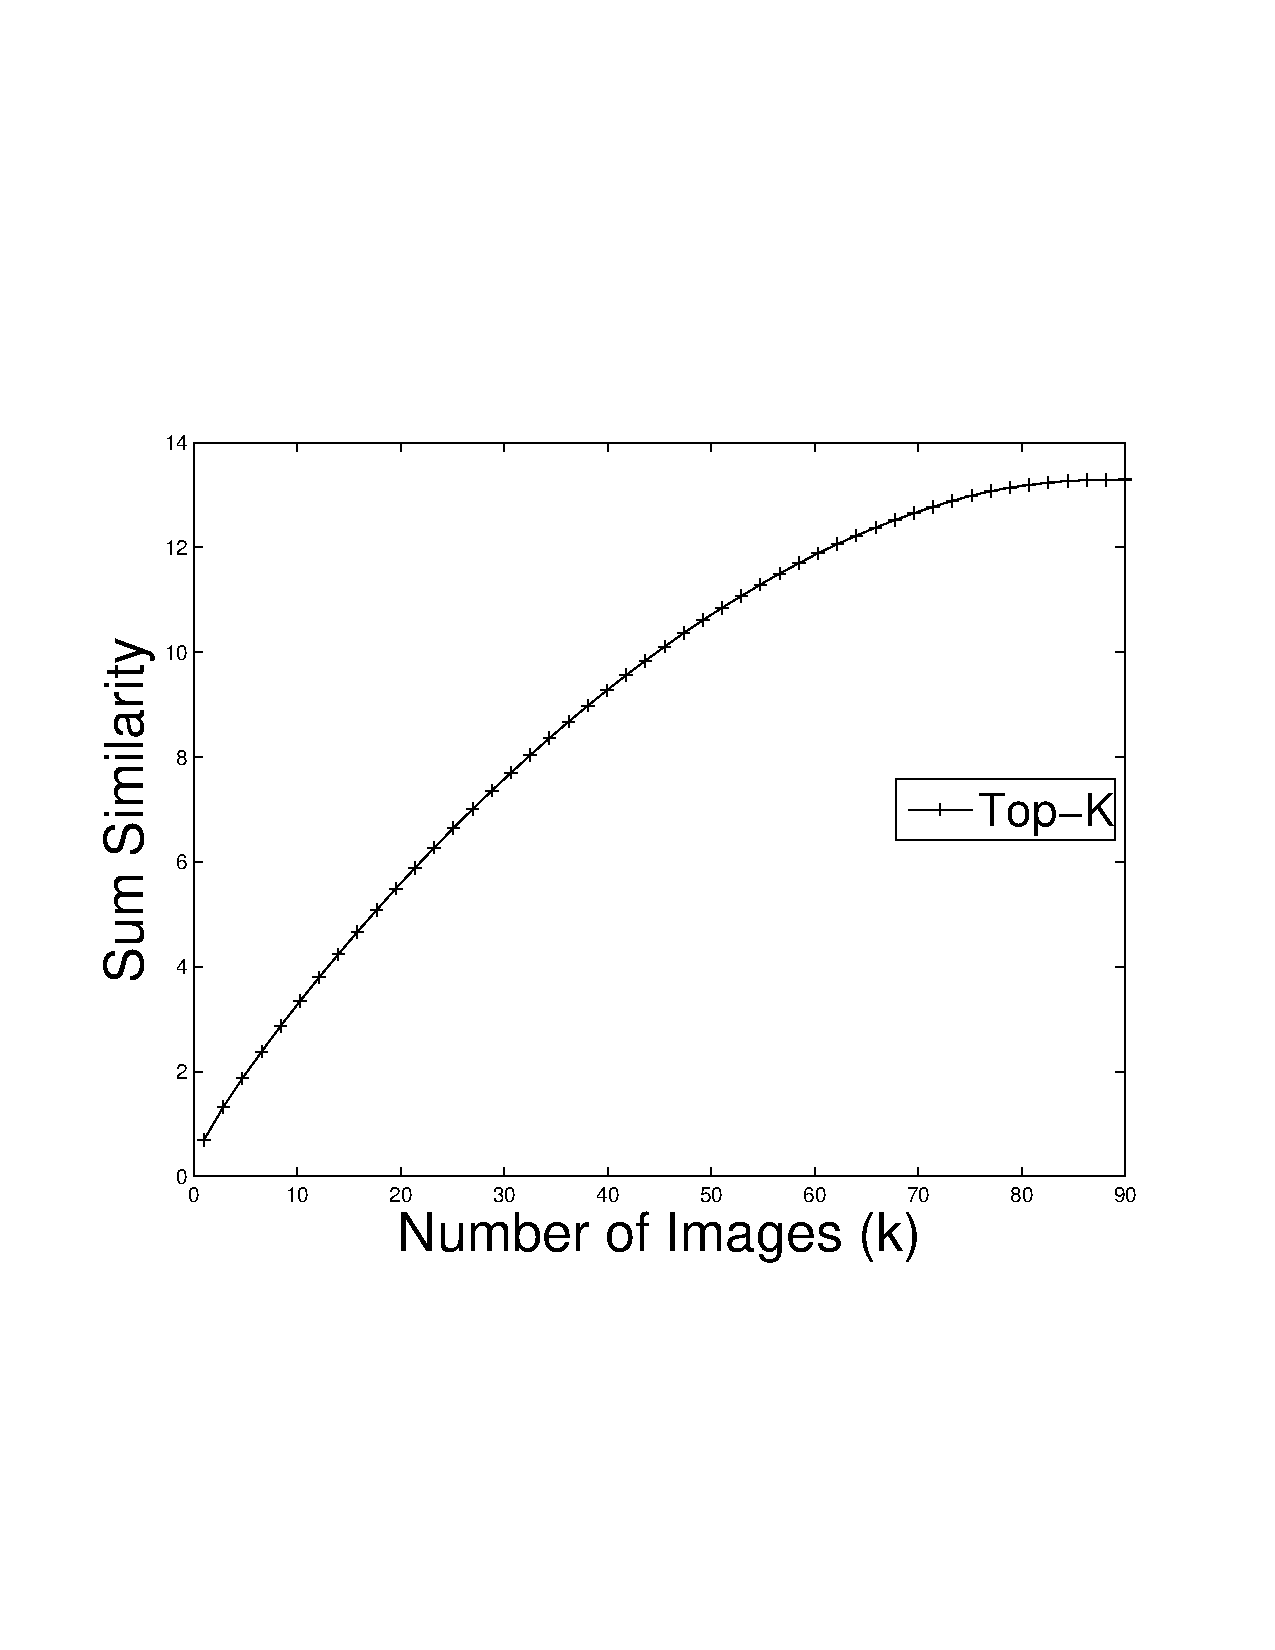
\includegraphics[clip=true, trim = 15mm 65mm 25mm 70mm, scale=0.23]{figures/USC_sumsim_topk.pdf}
        \label{fig:topkSumSim}
        }
    \subfigure[Top-K: Expected Sets Covered]{
        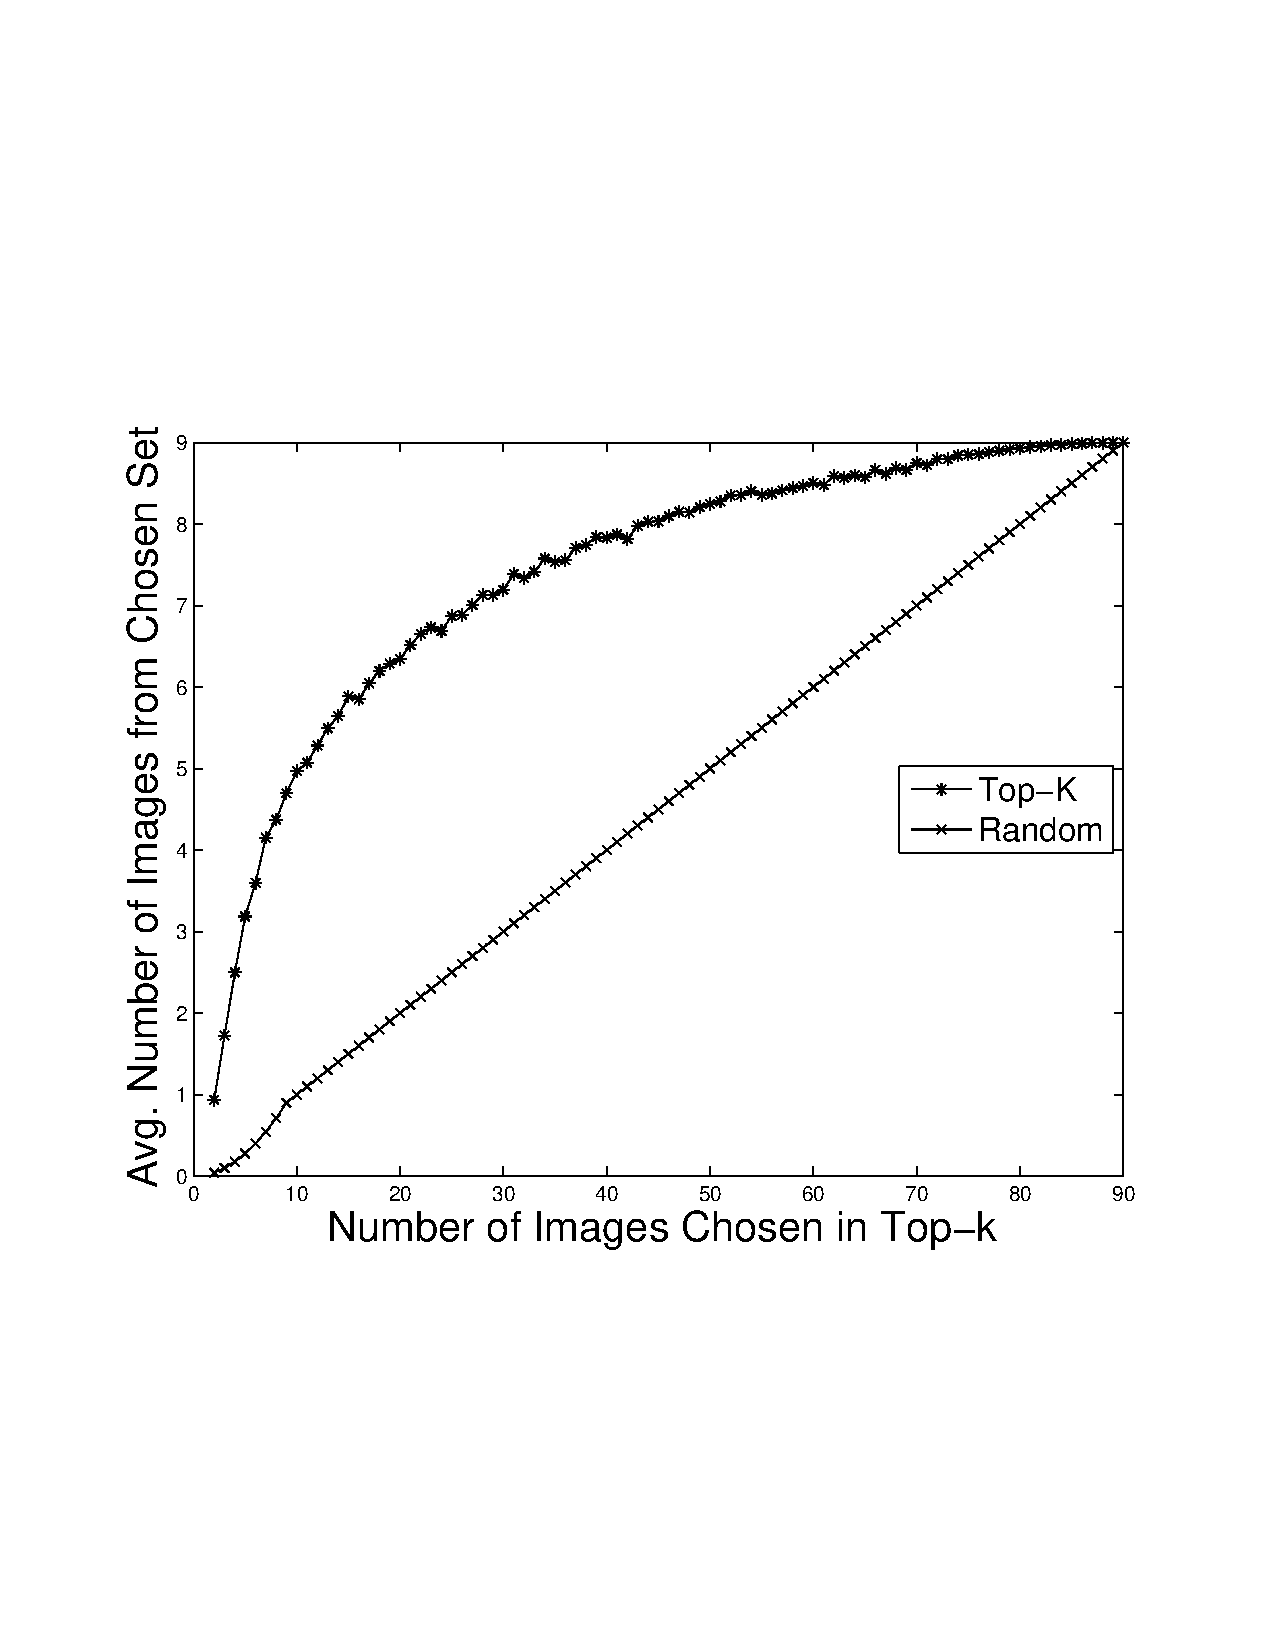
\includegraphics[clip=true, trim = 15mm 65mm 20mm 70mm, scale=0.23]{figures/topk/avg_num_matching.pdf}
        \label{fig:topkAvgNumSameSet}
        }
    \subfigure[Spanner: Sum Dissimilarity]{
        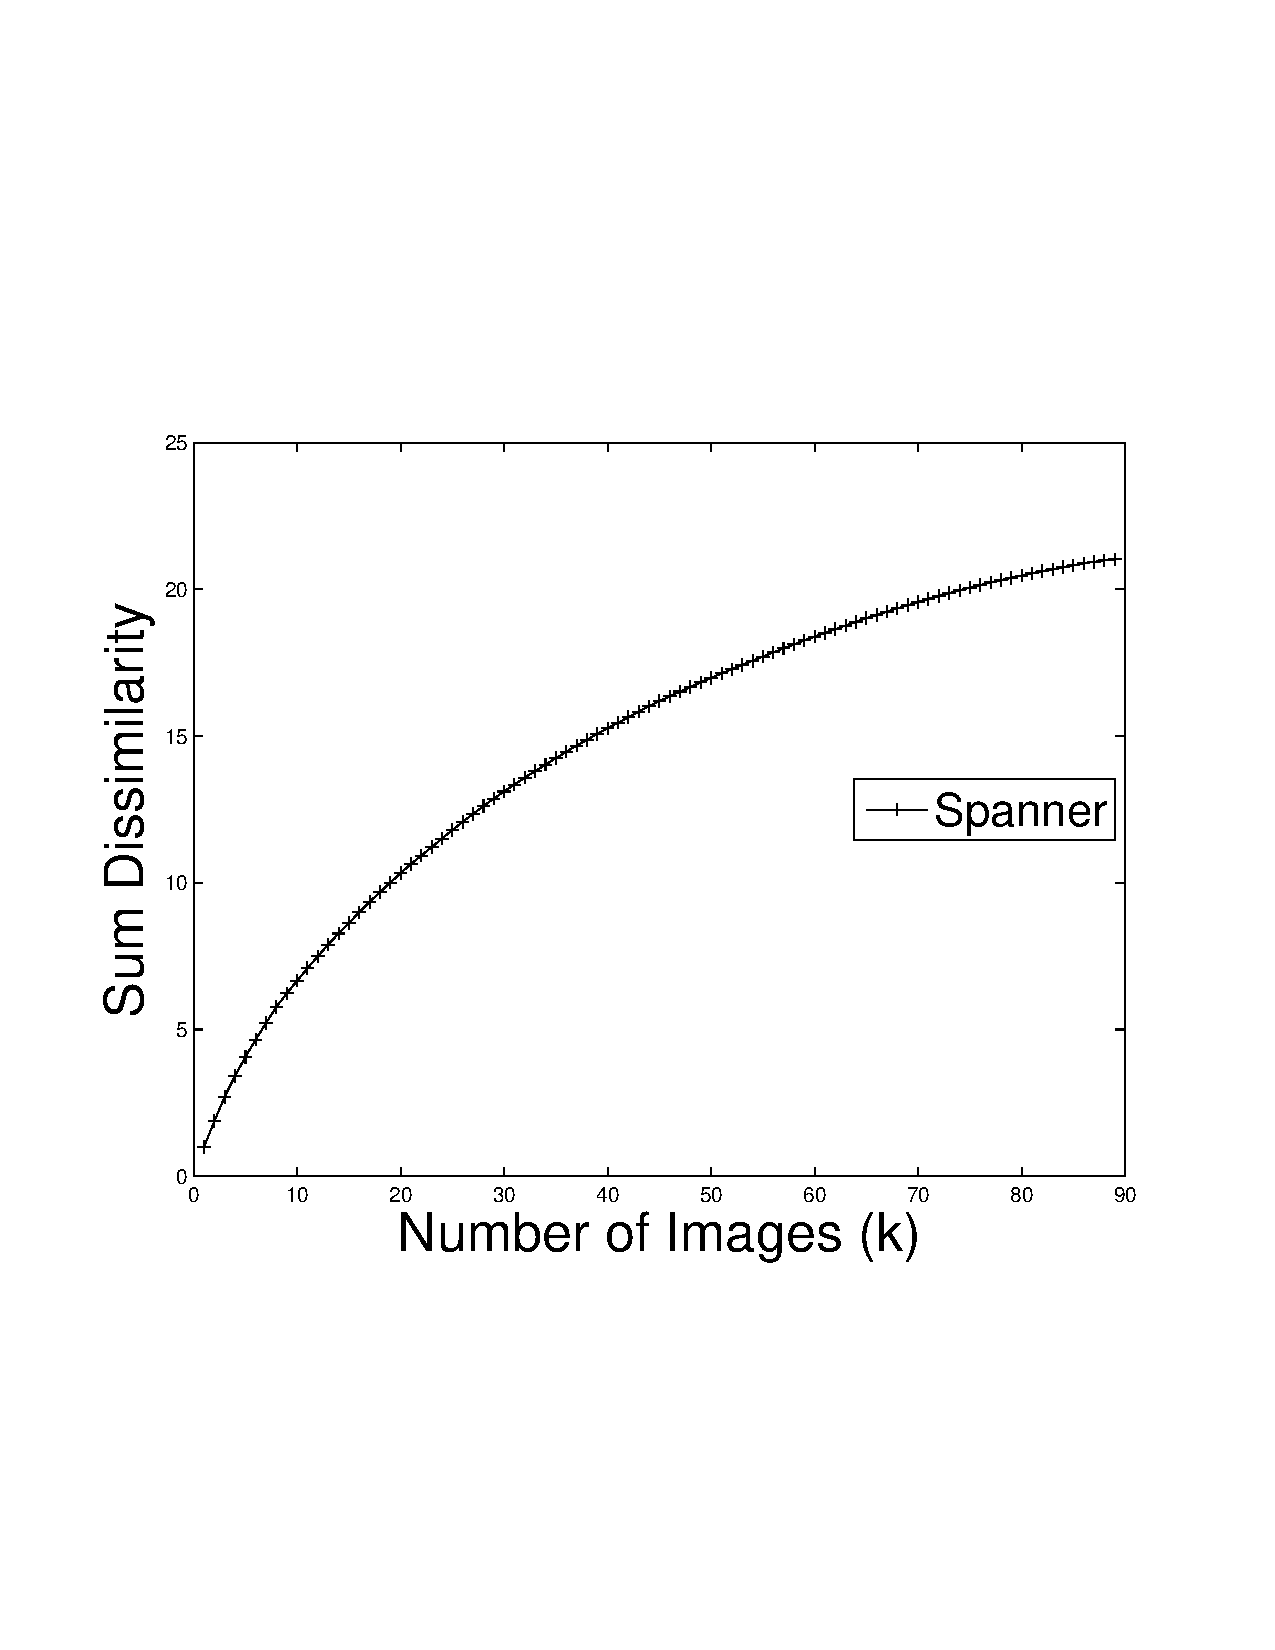
\includegraphics[clip=true, trim = 15mm 65mm 20mm 70mm, scale=0.23]{figures/spanner/spannerCumulativeDist.pdf}
        \label{fig:spanSumDissim}
        }
    \subfigure[Clustering: Prob. all Sets Covered]{
        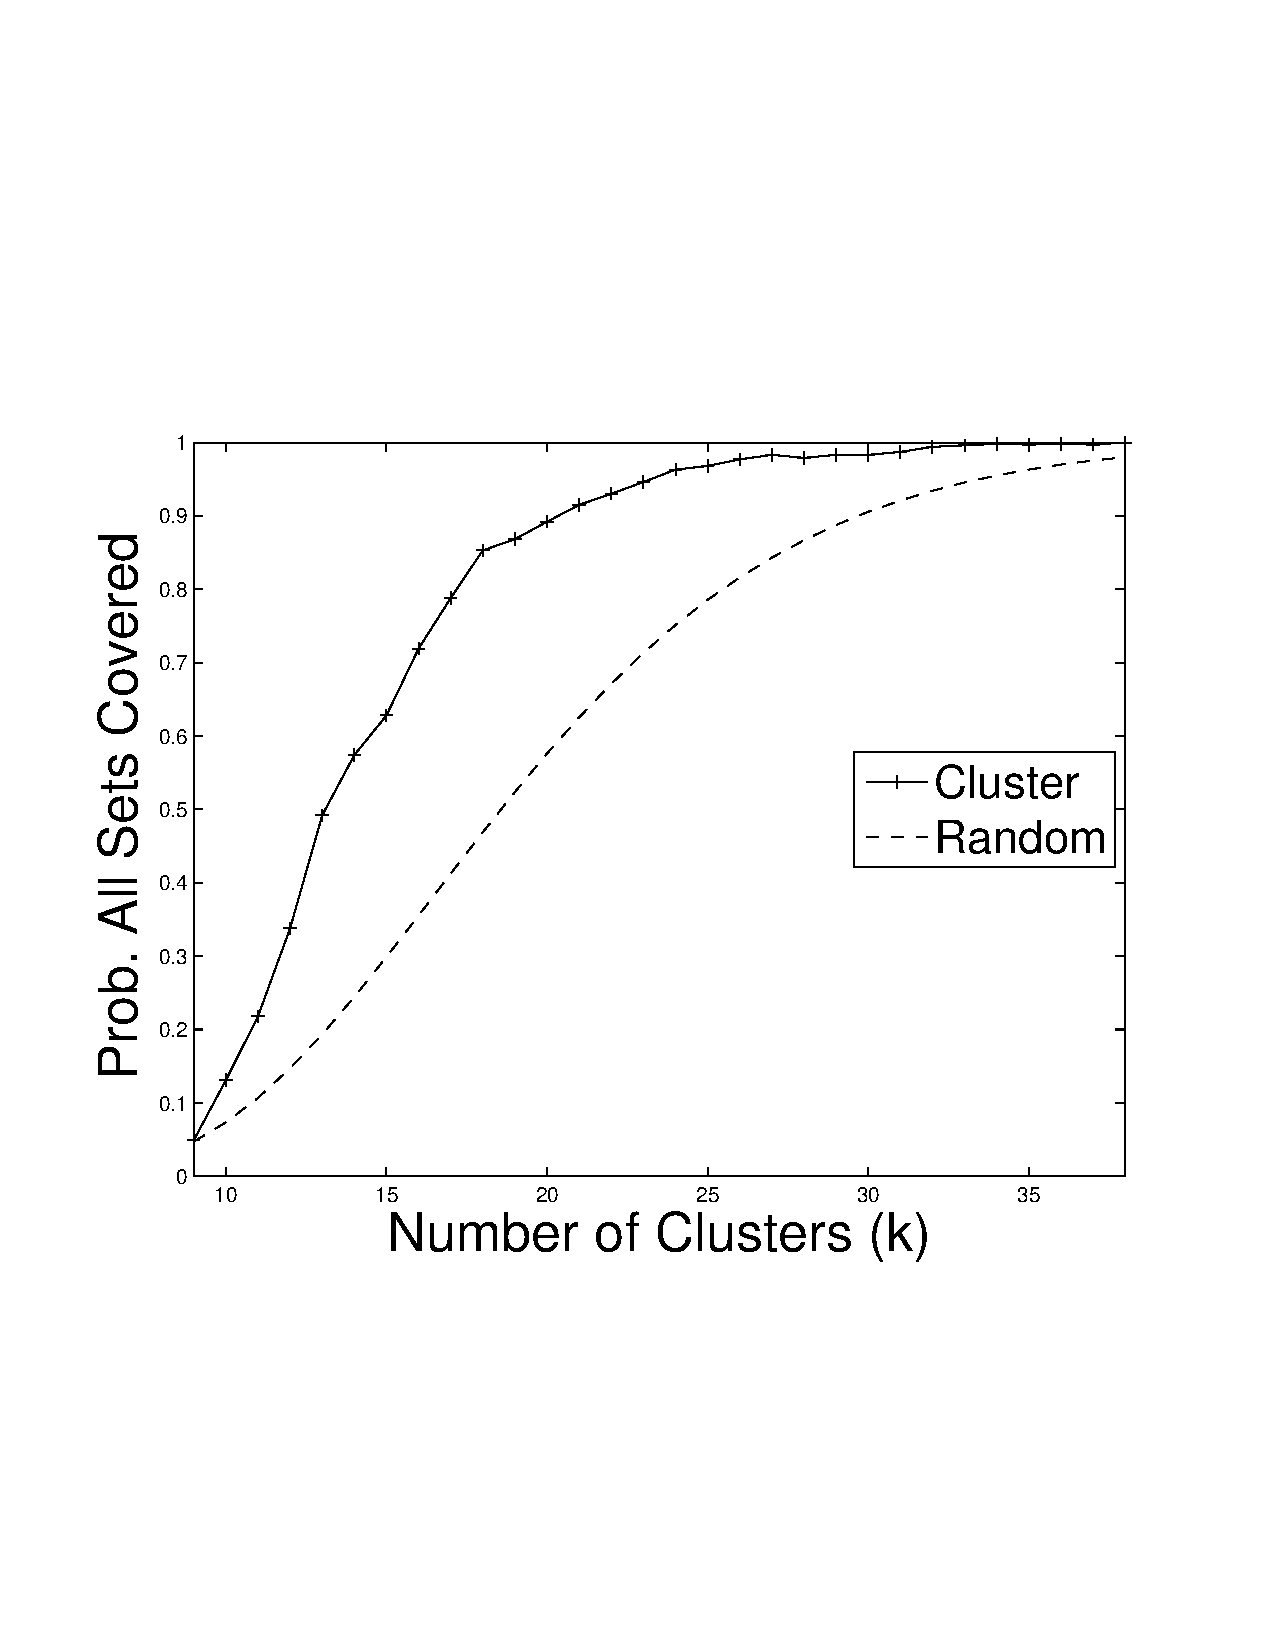
\includegraphics[clip=true, trim = 15mm 65mm 20mm 70mm, scale=0.23]{figures/cluster/perc_all_sets_covered_vary_k.pdf}
        \label{fig:clusterAvgNumSetsCov}
        }
        
        \vspace{-1mm}
   \caption{Completeness metrics for the three image selection algorithms. Each exhibits a diminishing return as more images are added.}
   \label{fig:completeness_exp_results}
   \vspace{-6mm}
\end{figure*}

QoI is a metric that can be defined for an application to give a more meaningful value to information by capturing attributes such as  timeliness, age/freshness, completeness, accuracy, precision, etc.  
For example, information that contributes to a decision-making process may only be useful if it arrives before the decision must be made, or it may have varying usefulness based on how similar or dissimilar it is to other data already collected.

The specific details of which attributes are considered and how they contribute to QoI is application-dependent.  The chosen QoI metrics are stored as a vector associated with a data item.  There are two ways to define QoI using that vector.  In one, a QoI function is defined that accepts the vector of metrics and provides a scalar value as an output like in  \cite{qoi_aware_mobile_apps,qoi_aware_trx_pol_time_vary_links} and many others.  In the second, as explained in \cite{qoi_aware_tactical_mil_nets}, a vector of minimum values for each QoI metric can be specified, and data can be evaluated based on whether it satisfies all of the QoI requirements or not.  We choose the latter method of determining QoI and focus on establishing the edges of QoI satisfiability for the vector of metrics, which defines the boundaries of maximum achievable QoI regions in the metric space.

We choose to use two QoI attributes, one that is time-based and one that is information-content-based.  The first attribute, whose importance has already been described, is timeliness, $T$, of data.  For the second attribute, we present a notion of \emph{completeness}, $C$, which we show can be defined multiple ways, depending on the context.  Together, a QoI requirement of $\mathbf{q} = \{C,T\}$ specifies a quantity of data that must be delivered as well as a deadline by which it must arrive to be useful.  While timeliness is not necessarily a new concept, completeness is less well defined.  Therefore, we identify three image selection algorithms, one that selects images based on similarity and two that select images based on diversity, and show how they can be evaluated with completeness.

\subsection{Image Selection Algorithms}

As a motivating example, we choose a network in which nodes store photographs that are to be exchanged or collected at one or more data sinks.  This example covers surveillance missions of military tactical networks or camera sensor networks.  Without adopting any one specific application, we present two query algorithms from \cite{mediascope}, one that helps return images similar to a target, and one that helps return a diverse set of images.  We also present ways to measure the completeness of each, providing a quantified value of a QoI metric.

Each of these queries require measuring the similarity or dissimilarity of two images.  To get a similarity measurement, we use the same choice as was shown to be effective in \cite{mediascope}.  This similarity is based on a technique called Color and Edge Directivity Descriptor (CEDD) \cite{2008cedd}, which uses qualities inherent to a photograph like lightness, contrast, and color.  The similarity between two images can then be given as a scalar by calculating the \emph{Tanimoto Similarity} \cite{tanimoto} between their CEDD vectors.  The dissimilarity value is simply defined as $1$ minus the similarity.

\subsubsection{Selecting Similar Images}

The first type of query we introduce occurs when a user already has one image of a particular area or object of interest and would like to obtain similar images to get a more complete view of that specific scene or object.  For example, if a user has a picture of an unknown suspicious person entering a building, but the person is not identifiable from that image, it would be useful to collect more images that are similar to that one with the possibility that another picture may have a better view of the person in question that can be used for identification or more context.  Called {\bf Top-K}, the query algorithm used for this application will choose the $k$ images with the most similarity with respect to the target image.  

Considering the goal of the Top-K query, we can evaluate the completeness of the result in one of two ways.  First, we can use the similarity of the images as a value representing each image's effectiveness in providing a more complete view of the target object or scene.  If we sum the similarity of all $k$ images returned by the algorithm, we get a representation of completeness, which we naturally call \emph{Sum Similarity}.  While this measure of completeness is abstract, it can be refined in an actual implementation through testing and evaluating.  This definition of completeness is useful, though, because it can be applied without any predetermined knowledge of the environment or pool of images.  

Often, though, we can partition the environment in which the network operates into a number, $n$, of distinct settings or areas.  In those cases, we can utilize a second method of quantifying completeness.  Assume that each image belongs to one of these $n$ sets, %$Q_i$, 
related to the setting it depicts.  Naturally, then, when executing a Top-K query, the goal is for the algorithm to return images from the same set as the target image.  Completeness can then be given by the fraction of images returned that are in the same set as the target image.

\subsubsection{Selecting Diverse Images}

In contrast, given the set of all photographs available in the network, we might want to return the set of $k$ images that exhibits the most diversity, ideally providing a user with a good sampling, or \emph{complete view}, of available images.  For instance, such a result would be quite useful in a surveillance mission.  We present two query algorithms that can be used to achieve this goal.

One query that provides diverse images is known as the {\bf Spanner} of the set of known photographs.  For the Spanner algorithm, we employ a greedy algorithm similar to that in \cite{mediascope} to simplify implementation and to define a \emph{Sum Dissimilarity} metric.  Here, the algorithm first chooses the two images with the greatest dissimilarity between them from all available images.  Then, each successive image is chosen to be the one with the greatest minimum distance between it and all images already chosen, until $k$ images are selected.  This minimum distance between the image being selected and the images in the collected set is the value added to the running cumulative completeness metric of \emph{Sum Dissimilarity}.  Since the Spanner algorithm's goal is to provide images at the edges of the available feature space, the Sum Dissimilarity represents a measure of its completeness because a higher level of dissimilarity is providing a more complete view of the feature space.

The other query that can achieve a complete view over all images is {\bf Clustering}.  In the Clustering algorithm, all images are separated into a $k$ clusters based on their pairwise distances using any version of a k-means clustering algorithm, where $k$ is given by the user.  Then, the most central image from each cluster is returned.  
Here, assuming that the photographs of the same settings or objects of interest exhibit similar characteristics, Clustering should provide a complete view of the network's environment.

Both Spanner and Clustering algorithms can also be evaluated using the model in which the environment is split into $n$ sets.  With this model, we can define completeness as either the number of sets represented by at least one of the $k$ images returned or the probability of all $n$ sets being represented by at least one image when $k$ are returned.  Here, though, we only show results for the second definition.

\subsubsection{Experimental Results}

%%Top-K Sum Similarity
%\begin{figure} 
%\centering
%    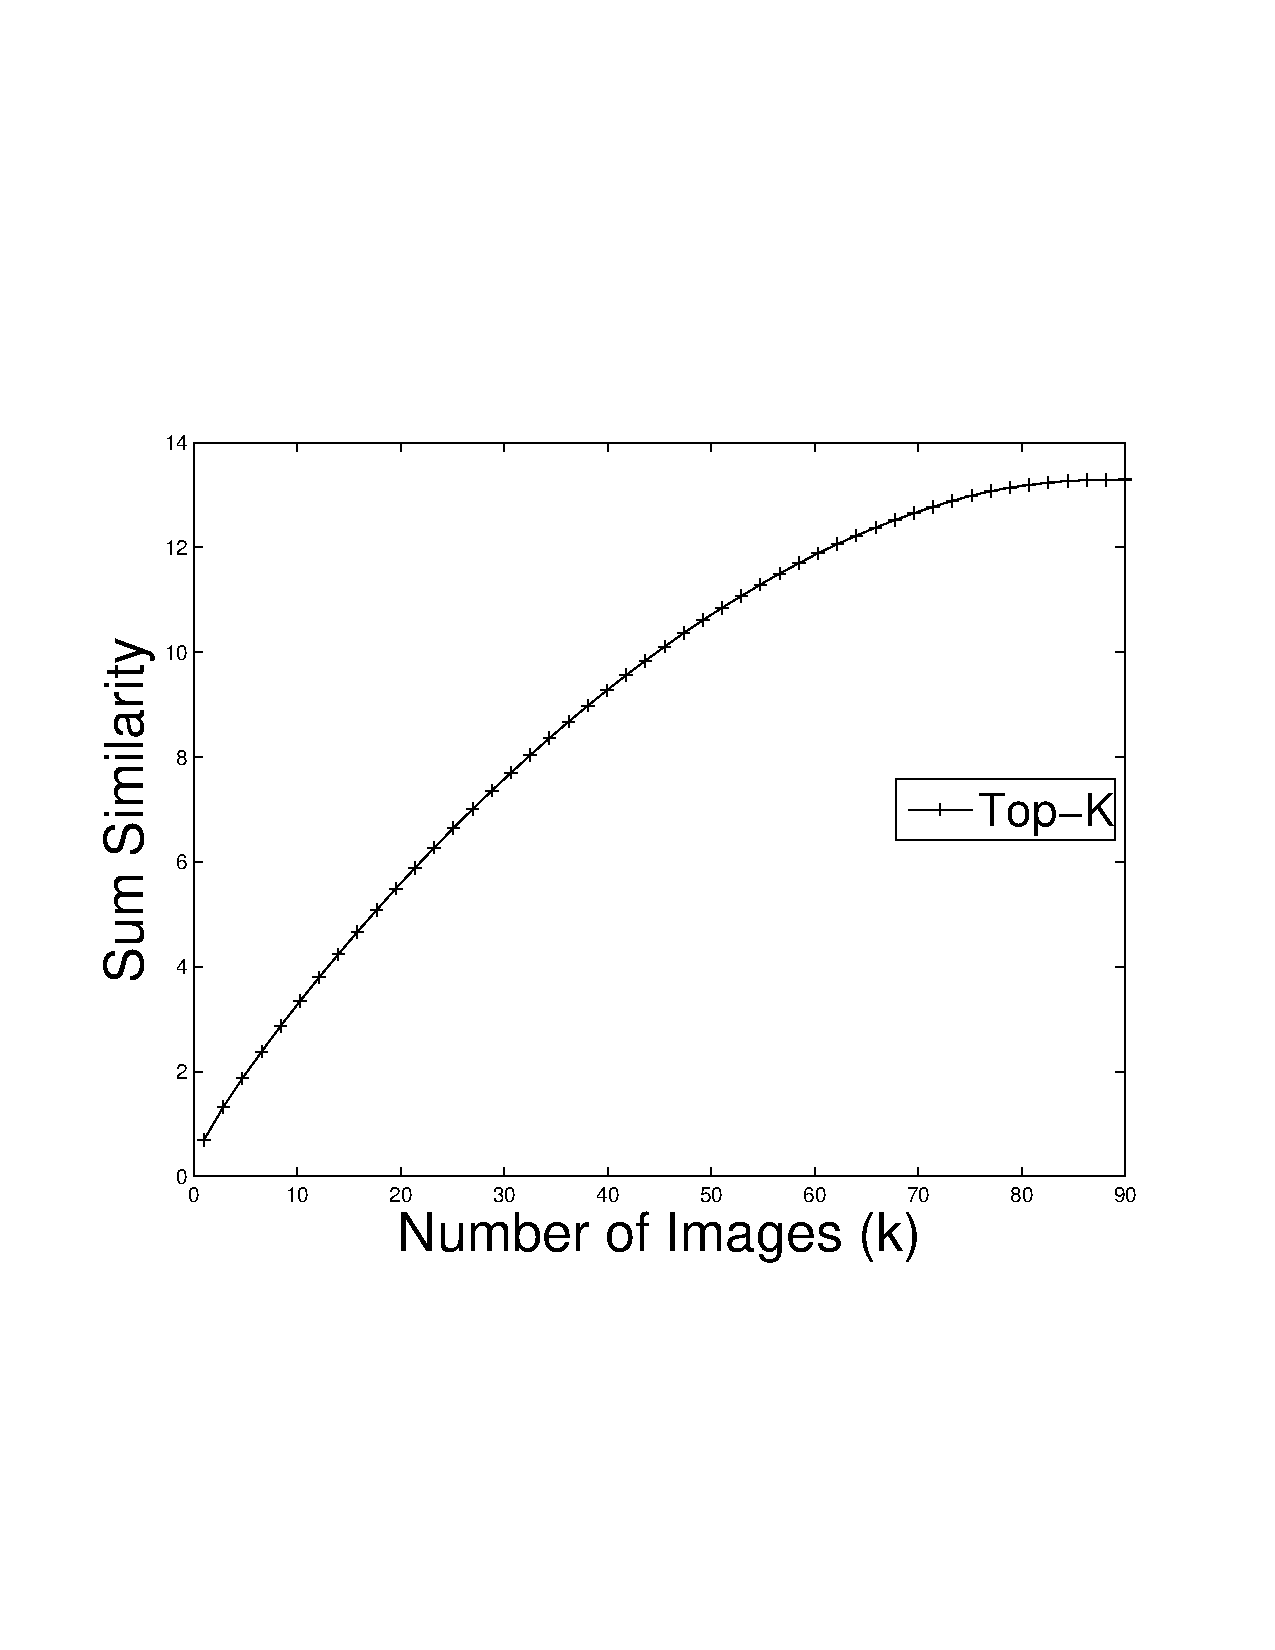
\includegraphics[clip=true, trim = 20mm 65mm 25mm 70mm, scale=0.35]{figures/USC_sumsim_topk.pdf}
%    \vspace{-4mm}
%    \label{fig:topkSumSim}
%    \vspace{-3mm}
%\end{figure}
%
%% Top-K Average Number from Same Set Returned
%\begin{figure} 
%\centering
%    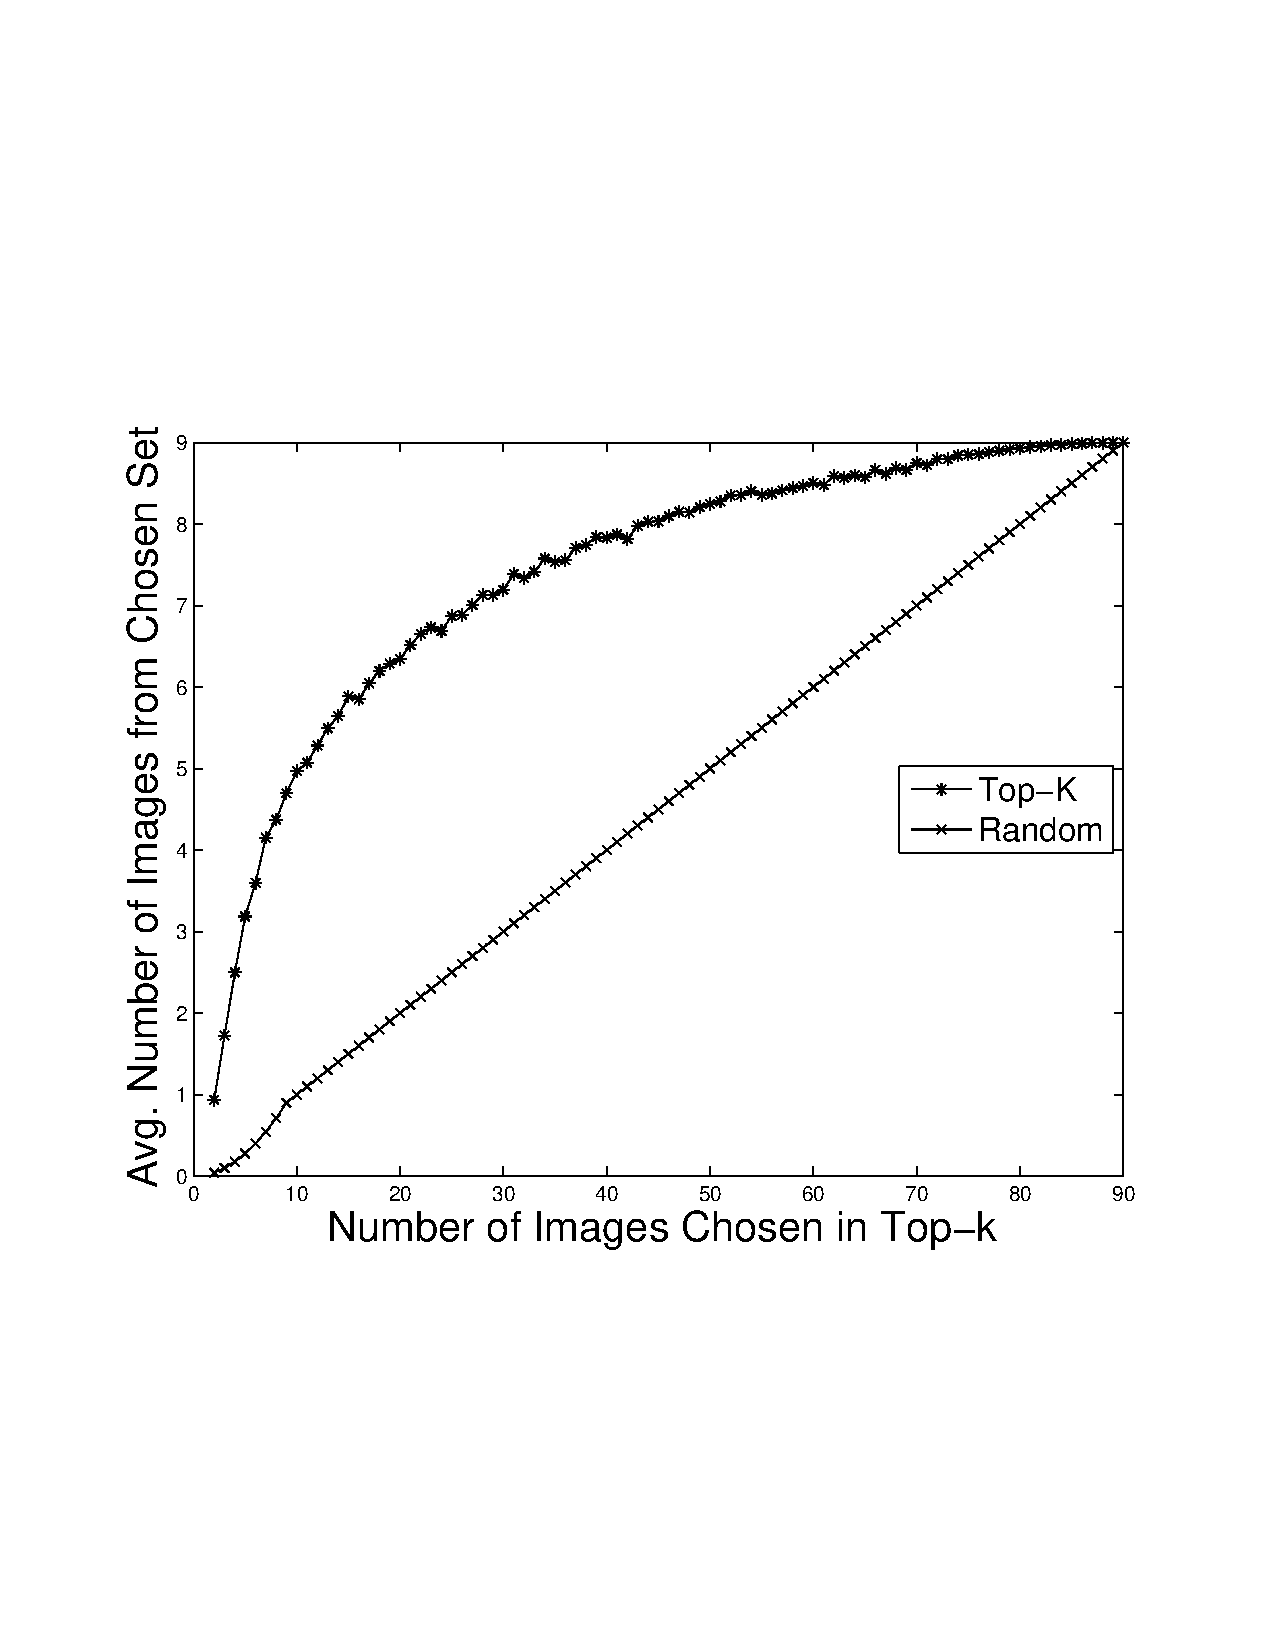
\includegraphics[clip=true, trim = 15mm 65mm 20mm 70mm, scale=0.35]{figures/topk/avg_num_matching.pdf}
%    \vspace{-3mm}
%    \caption{Top-K algorithm performs returns more images from target set than random, but also exhibits diminishing returns as $k$ increases.}
%    \label{fig:topkAvgNumSameSet}
%    \vspace{-6mm}
%\end{figure}

To provide example values of these completeness metric definitions, experiments applying each query algorithm were run on a set of pictures taken at $n = 9$ different settings around the Penn State campus.  Each of these $9$ settings is of a pictorially different area, e.g. a particular building, a downtown street, or a lawn setting, and over $20$ images of each was taken.  Then, for individual trials, $10$ images from each set were randomly selected to create an image pool of $90$ pictures.  The three algorithms were run over these $90$ images, with the target image being randomly selected in the case of Top-K.  Results for each of the different completeness metrics were averaged over $1,000$ trials are shown in Figures \ref{fig:topkSumSim} to \ref{fig:clusterAvgNumSetsCov}.

Figure \ref{fig:topkSumSim} shows the average sum similarity of images returned by the Top-K algorithm.  Figure \ref{fig:topkAvgNumSameSet} provides the second definition of completeness for the Top-K algorithm, the number of images matching the set that the target image was randomly chosen from.  
Completeness results when dissimilarity is the objective are shown in Figures \ref{fig:spanSumDissim} and \ref{fig:clusterAvgNumSetsCov}.  Specifically, Figure \ref{fig:spanSumDissim} depicts the average Sum Dissimilarity returned by the Spanner algorithm, and 
Figure \ref{fig:clusterAvgNumSetsCov} represents the empirical probability of all $9$ sets being represented in the $k$ returned images.   For reference, we also include expected values for the metrics in Figures \ref{fig:topkAvgNumSameSet} and \ref{fig:clusterAvgNumSetsCov} if the images were selected from the entire image pool at random, i.e., without regard for image similarity or dissimilarity.  

All of these figures exhibit the diminishing returns of completeness as more images are collected.  This effect is important because it visually shows how QoI differs from throughput.  As seen in these graphs, transmission of successive images does not result in a linear gain in completeness.  For example, in Figure \ref{fig:topkAvgNumSameSet}, it is evident that a value of only $k \approx 10$ is needed to collect $5$ images matching the target content, while collecting an additional $2$ from the same set usually requires collecting over twice that number of pictures.  

As a second example, Figure \ref{fig:clusterAvgNumSetsCov} shows that jumping from $k=10$ to $k=20$, the likelihood of capturing at least one image of every setting grows substantially from just over $10\%$ to approximately $90\%$.  To approach probabilities close to gaining that final $10\%$, however, requires a jump to $k\approx30$.  

%%Spanner Sum Dissimilarity
%\begin{figure} 
%\begin{centering}
%    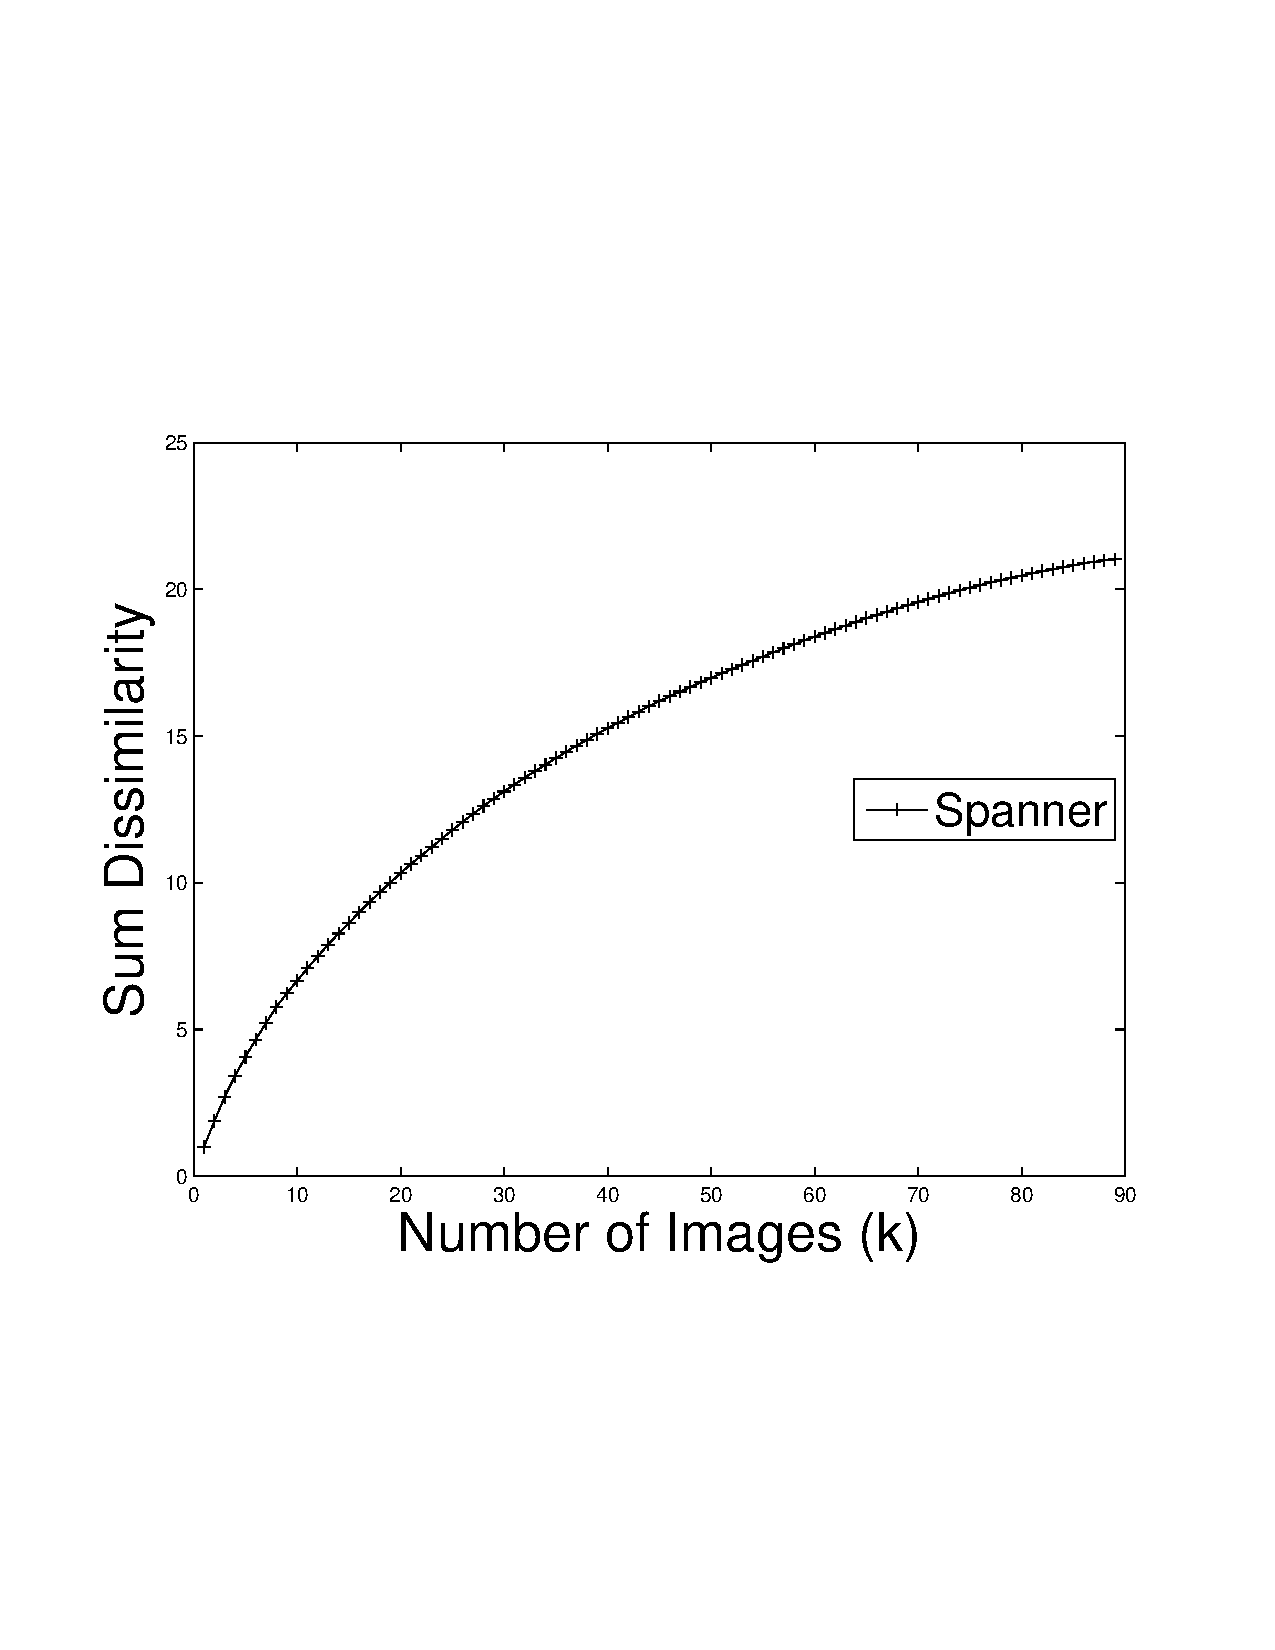
\includegraphics[clip=true, trim = 15mm 65mm 20mm 70mm, scale=0.35]{figures/spanner/spannerCumulativeDist.pdf}
%    \vspace{-3mm}
%    \caption{Diminishing returns on Sum Dissimilarity exhibited by the Spanner algorithm as more images are retrieved.}
%    \label{fig:spanSumDissim}
%    \vspace{-3mm}
%\end{centering}
%\end{figure}
%
%% Cluster Percentage All Sets Covered
%\begin{figure} 
%\begin{centering}
%    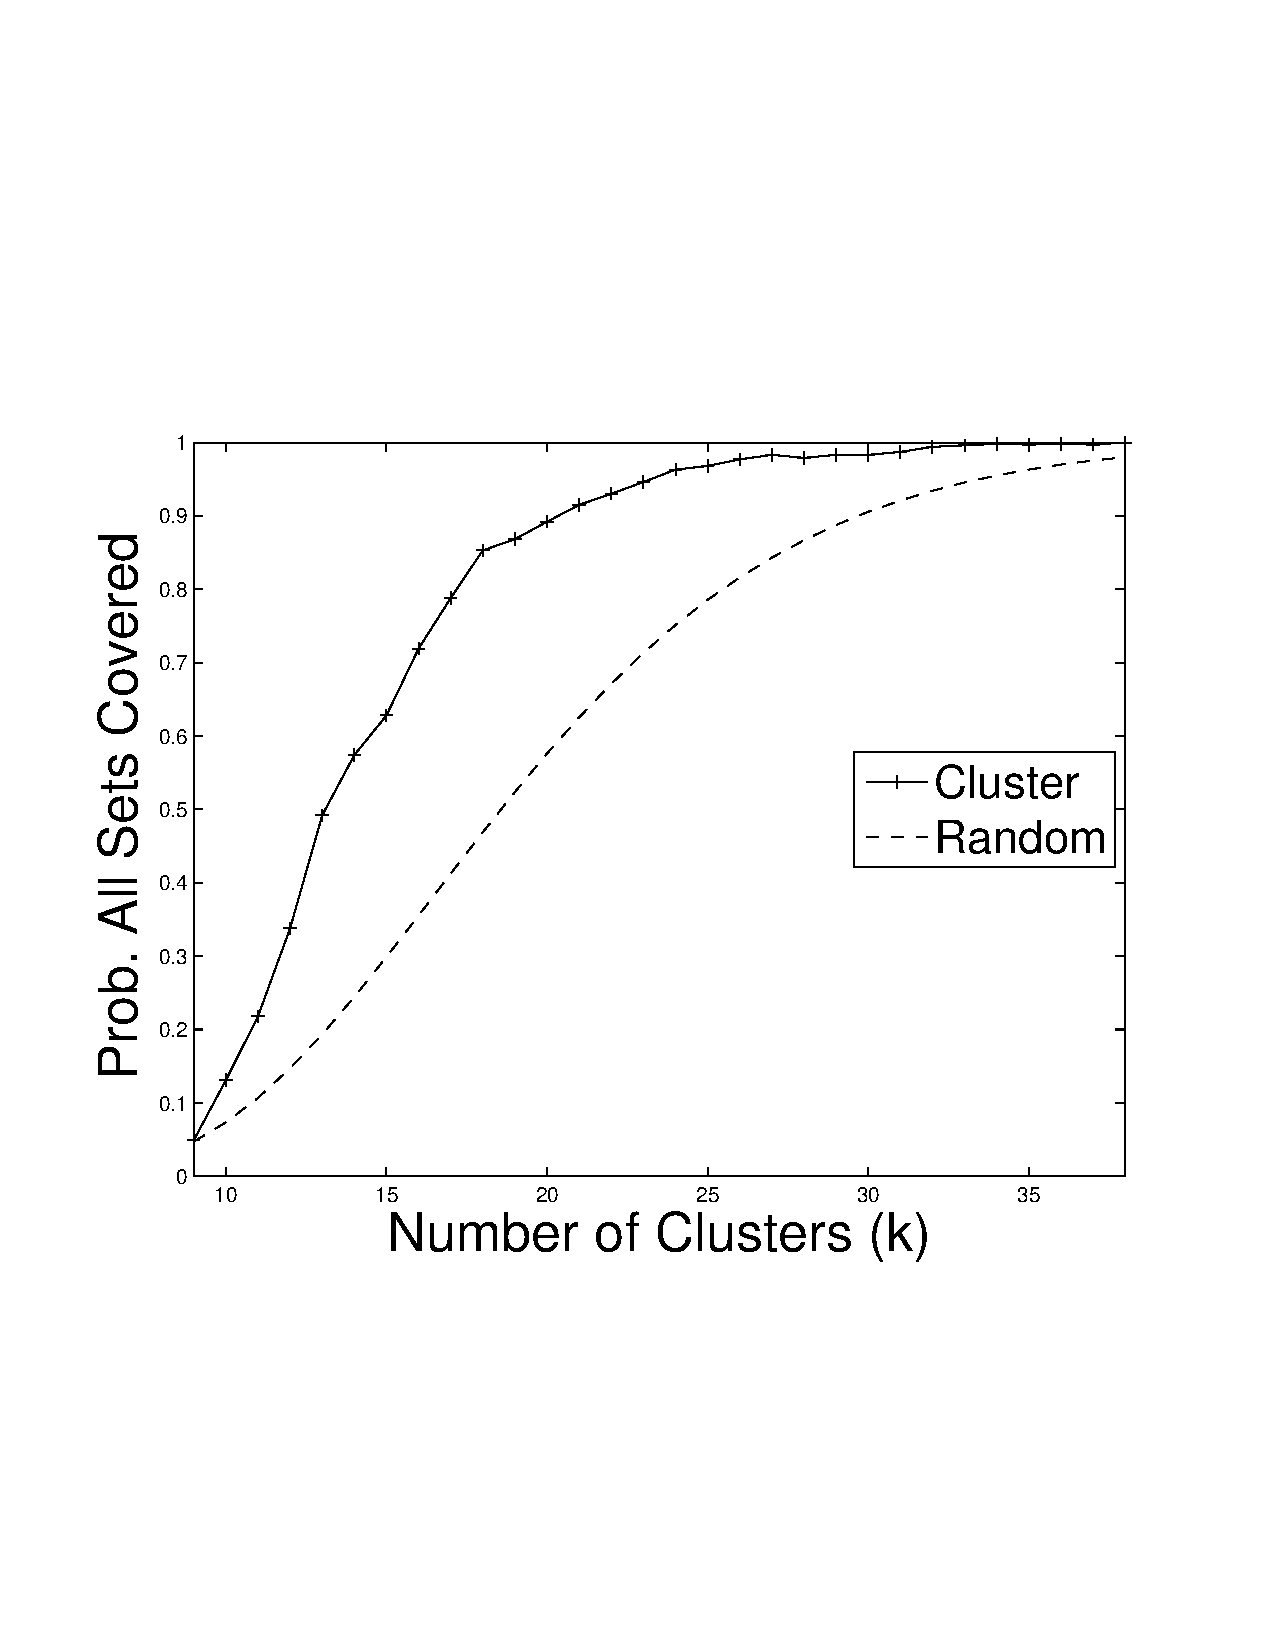
\includegraphics[clip=true, trim = 15mm 65mm 20mm 70mm, scale=0.35]{figures/cluster/perc_all_sets_covered_vary_k.pdf}
%    \vspace{-3mm}
%    \caption{Empirical probability of obtaining at least one image from every set as $k$ is increased with the Clustering algorithm.  A highly non-linear, diminishing returns effect is seen.}
%    \label{fig:clusterAvgNumSetsCov}
%    \vspace{-7mm}
%\end{centering}
%\end{figure}

The relationship between the number of images and completeness in each of these graphs also shows that obtaining a certain value of QoI or completeness requires a different number of images depending on the set available and their similarities.  We can denote the number of images required to achieve a level of completeness, $C$, as $k_{req} = Q(C)$.  This relationship will be useful later in determining capacity and scalability limits.

\subsection{Further Discussion of QoI}
We have defined and provided examples for a number of ways that completeness can be defined and used to obtain a concrete data requirement from a contextual QoI requirement.  Throughout the rest of the paper, we mainly use sum similarity as the completeness metric, but any of the definitions of completeness used here, or any other QoI requirement that can be translated into a data requirement, for that matter, can be used in the following formulation in Section \ref{sec:qoi_scalability}.

Also, note that QoI and its usage in understanding networks is not exclusive to these metrics and applications.  On the contrary, the model used in the capacity and scalability analysis of Section \ref{sec:qoi_scalability} is meant to be an in-depth example of this concept.  Modifications to account for different data size requirements should be quite straightforward, and extensions to other time-based metrics should be possible with careful extensions to the framework.

Finally, while metadata associated with photographs may be useful in obtaining similar goals to those given in this section, relying on such information is problematic because metadata is not guaranteed to be available, and it is not as universally applicable as content-based retrieval.  For example, tags describing the image contents would require users to participate by entering this information, which is a time-consuming and unreliable step that users are likely to ignore.  Location and time stamps may be automatically applied by the device allowing an application to filter images accordingly, but these tags often do not account for factors such as the direction of the camera or obstructed views.  Content-based processing of these images, though, can be applied to any set of images.





%
\section{Symptotics Framework}
\label{sec:symptotics_bckgrnd}

Here, we provide an overview of the network scalability framework.



\section{QoI Scalability}
\label{sec:qoi_scalability}

\begin{figure}
\centering
    \subfigure[$TF = 2$, $CF = 3$, $DF = 1$]{
        \includegraphics[scale=0.28, clip=true, trim=5mm 0mm 5mm 0mm, valign=t]{delay_expl_fig_a.pdf}
        \label{fig:delay_expl_fig_3}
        }
    \subfigure[$TF = 2$, $CF = 3$, $DF = 2$]{
        \includegraphics[scale=0.28, valign=t]{delay_expl_fig_b.pdf}
        \label{fig:delay_expl_fig_4}
        }

   \caption{Example of line network using TDMA highlighting source of delays. (Node labels are TDMA slot assignments.)}
   \label{fig:both_delay_figures}
   \vspace{-5mm}
\end{figure}

Given the nonlinear returns of completeness and importance of timeliness outlined in the previous section, we contend that simply establishing the highest average supportable rate should not be the only goal of a QoI-aware network.  With this knowledge, we set the goal of determining the capacity of a network (and relatedly, the scalability achievable) with respect to {\em QoI requirements}, instead of the maximum throughput.  

\subsection{QoI Satisfiability Framework}
In order to establish the framework, we examine an arbitrary flow, $F_1$, in the network that has a QoI requirement of $\mathbf{q} = \{C, T\}$, where $C$ is the minimum required completeness metric of choice, such as sum similarity as explained above, and $T$ is the required timeliness.  This flow will have a data size requirement, which is given by a chosen QoI function $Q(C)$ like those discussed in Section \ref{sec:qoi_model}.  Using the example applications from \ref{sec:qoi_model}, for example, $Q(C)$ can return the number of images, $k_{req}$, required to achieve the requested completeness $C$ according to established relations like those in Section \ref{sec:qoi_model}.  Assuming each image has an average size of $I_S$, then we can also use $B$ to describe the total number of bits required by the flow, $B=k_{req}*I_S$.  To match realistic network implications, we assume this data will be transmitted in a series of packets with size $P_S$ bits each.  The number of packets per flow, then, is simply $P_N = \lceil B/P_S \rceil$.  We assume that each node in the network can transmit at $W$ bits per second when it is allocated media access.

Our goal is to establish the limits at which this arbitrary flow on average can no longer be completed with the QoI requirements satisfied.  We build and explain our model for achieving this goal by working through an example TDMA line network, a portion of which is shown in Figures \ref{fig:delay_expl_fig_3} and \ref{fig:delay_expl_fig_4} (We discuss addressing non-TDMA networks in Section \ref{sec:discussion}).  In this network, we assume a simple 3-slot TDMA scheme, which allows each node equal time access to the medium and removes any potential interference or hidden terminal issues.  Each node in the figure is labeled with its allocated slot.  For simplicity, we will assume that one slot is appropriately sized to transmit a single packet, i.e., $T_{slot} = P_S/W$ and that packets use static routes calculated beforehand such that the overhead is not a consideration here.

Now, two factors, $D_1$ and $D_2$, contribute to the total delay of completing $F_1$.  The first contributor, $D_1$, is the end to end delay incurred by sending the $B$ bits across the entire path.  To quantify this delay, we must consider several factors beyond just the available bandwidth and number of packets.  First, each node can only utilize its allotted channel time, creating a Channel Factor of $CF = N_{frame}/N_{i}$, where $N_{i}$ is the number of slots allocated to node $i$ and $N_{frame}$ is the total number of slots in each frame.  In this case, $N_{i} = 1, \forall i$ and $N_{frame} = 3$.  The second factor to consider for $D_1$ is the fraction of allocated slots that are utilized by the node to serve flows other than $F_1$ that are either originating in or being routed through nodes on the path of flow $F_1$.  We call the total number of flows competing at node $i$ the Traffic Factor, $TF_i$, of that node.  For any flow, the maximum contributor to delay is the node along the path with the maximum $TF_i$, which we will just call $TF$ here.  Incorporating these considerations into a calculation for $D_1$, we achieve the following expression


\begin{equation}
	D_1 = T_{slot} \cdot P_N \cdot CF \cdot TF
\end{equation}
%\begin{figure}
%\begin{centering}
%    \includegraphics[scale=0.33]{figures/delay_limit_expl/delay_expl_fig_a.pdf}
%    \caption{Example of line network using TDMA highlighting source of delays, $D_1$ and $D_2$.  Here, $TF = 2$, $CF = 3$, and $DF = 1$. }
%    \label{fig:delay_expl_fig_3}
%    \vspace{-3mm}
%\end{centering}
%\end{figure}

Figure \ref{fig:delay_expl_fig_3} depicts the delay of $D_1$ in a simple case of only two flows, $F_1$ and $F_2$, being present, in which case $TF = 2$.  In this example we use flows that consist of only $2$ ($F_{i-j}$ is packet $j$ in flow $i$) packets to portray the delay.  In most real applications, $P_N$ will be much larger, making $D_1$ a good approximation of this delay component.

%\begin{figure}
%\begin{centering}
%    \includegraphics[scale=0.35]{figures/delay_limit_expl/delay_expl_fig_b.pdf}
%    \caption{In the opposite direction, $DF = 2$. ($TF$ and $CF$ are unchanged here.)}
%    \label{fig:delay_expl_fig_4}
%\vspace{-5mm}
%\end{centering}
%\end{figure}

The second delay that exists is due to multi-hop propagation of packets.  This delay is simply the time for a single packet to traverse the path length.  Note that this delay is not necessarily just the path length multiplied by $T_{slot}$, because of possible queuing delays and/or ordering constraints.  We show here how ordering constraints impact this TDMA network.  A node cannot forward a packet from the flow until it receives that packet from the previous hop.  In our line network example, when the direction of the flow matches the nodes' schedule of slots $1-2-3-1-2-3$, as in Figure \ref{fig:delay_expl_fig_3}, each successive node receives a packet on the time slot before it is scheduled, resulting in no extra delay.  For a flow in the opposite direction, though, where nodes are scheduled $3-2-1-3-2-1$, as in Figure \ref{fig:delay_expl_fig_4}, the first slot $1$ is not utilized, because the first node scheduled in time slot $1$ has not yet received a packet in the flow.  Every other slot is wasted, on average, for the initialization of the flow, resulting in approximately twice the delay.  We will use a term that we call the \emph{Delay Factor}, or $DF$, to account for this effect where it exists.

The multi-hop propagation delay, then, is modeled by

\begin{equation}
	D_2 = T_{slot} \cdot DF \cdot (PL - 1)
\end{equation}
where $PL$ is the average path length.

We note several points about this delay factor.  First, in a loaded network, the nodes can and will serve other flows while awaiting the arrival of packets in this flow of focus.  That utilized bandwidth does not, however, preclude this $DF$ impact on delay for the flow of interest, $F_1$.  Any node cannot serve $F_1$ until a packet from that flow has been received.  Second, this delay is only accounted for once per flow because all other packets are pipelined.  All other packets' delay is captured by the end to end delay, $D_1$.  This effect is best illustrated by examining the difference between $D_2$ in Figures \ref{fig:delay_expl_fig_3} and \ref{fig:delay_expl_fig_4}.  Here, we see the multi-hop propagation requires twice the number of slots because every other slot is unused in $F_1$'s propagation.  
%Note that these unused slots may be used by the nodes to transmit packets from a different flow, so the bandwidth may be utilized, but since it cannot be used for flow $F_1$, the delay for this flow is still impacted by $DF$.

To calculate a $DF$ for an entire network, we can calculate a $DF$ for each possible sample path and find the average of these values.  For example, in the case of the line network with a $3$-slot schedule, $DF = 1$ in the direction for Figure \ref{fig:delay_expl_fig_3} and $DF = 2$ in the opposite direction shown in Figure \ref{fig:delay_expl_fig_4}, so the average $DF$ used to approximate average delay in the network is $DF_{line-avg}=1.5$.  

By combining the two components of delay, we can give a relation for a network that will successfully achieve an average flow's data and timeliness requirements:

\vspace{-2mm}
\begin{equation*}
	D_1 + D_2 \leq T 
\end{equation*}
\begin{equation*}
	T_{slot} \cdot P_N \cdot CF \cdot TF + T_{slot} \cdot DF \cdot (PL-1) \leq T
\end{equation*}

Recalling that the time of a slot is determined by the size of a packet, $P_S$, and available channel rate, $W$, in the relation $T_{slot} = P_S/W$, we can substitute to get
\begin{equation*}
	\frac{P_S}{W} \cdot P_N \cdot CF \cdot TF + \frac{P_S}{W} \cdot DF \cdot (PL-1) \leq T
\end{equation*}
Finally, substituting the total number of bits required for a flow $P_S \cdot P_N =  k_{req} \cdot I_S$ (where $k_{req}$ is given by a function of required QoI), and rearranging this inequality, we can obtain a cleaner view of each parameter's impact on network limits:

\vspace{-2mm}
\begin{equation}
	W \cdot T - k_{req} \cdot I_S \cdot CF \cdot TF - P_S \cdot DF \cdot (PL-1) \geq 0	
	\label{eq:general_scal}
\end{equation}

Every network will have its own set of parameters that can be substituted into this general formula, providing a tool to approximate limitations and sensitivity to changes in specific parameters.  To show this usefulness concretely, we provide derived values for a TDMA-based wireless network with several basic topologies.


\begin{figure*}[]
\centering
    \subfigure[Clique Network, $I_S = 9 MB$]{
        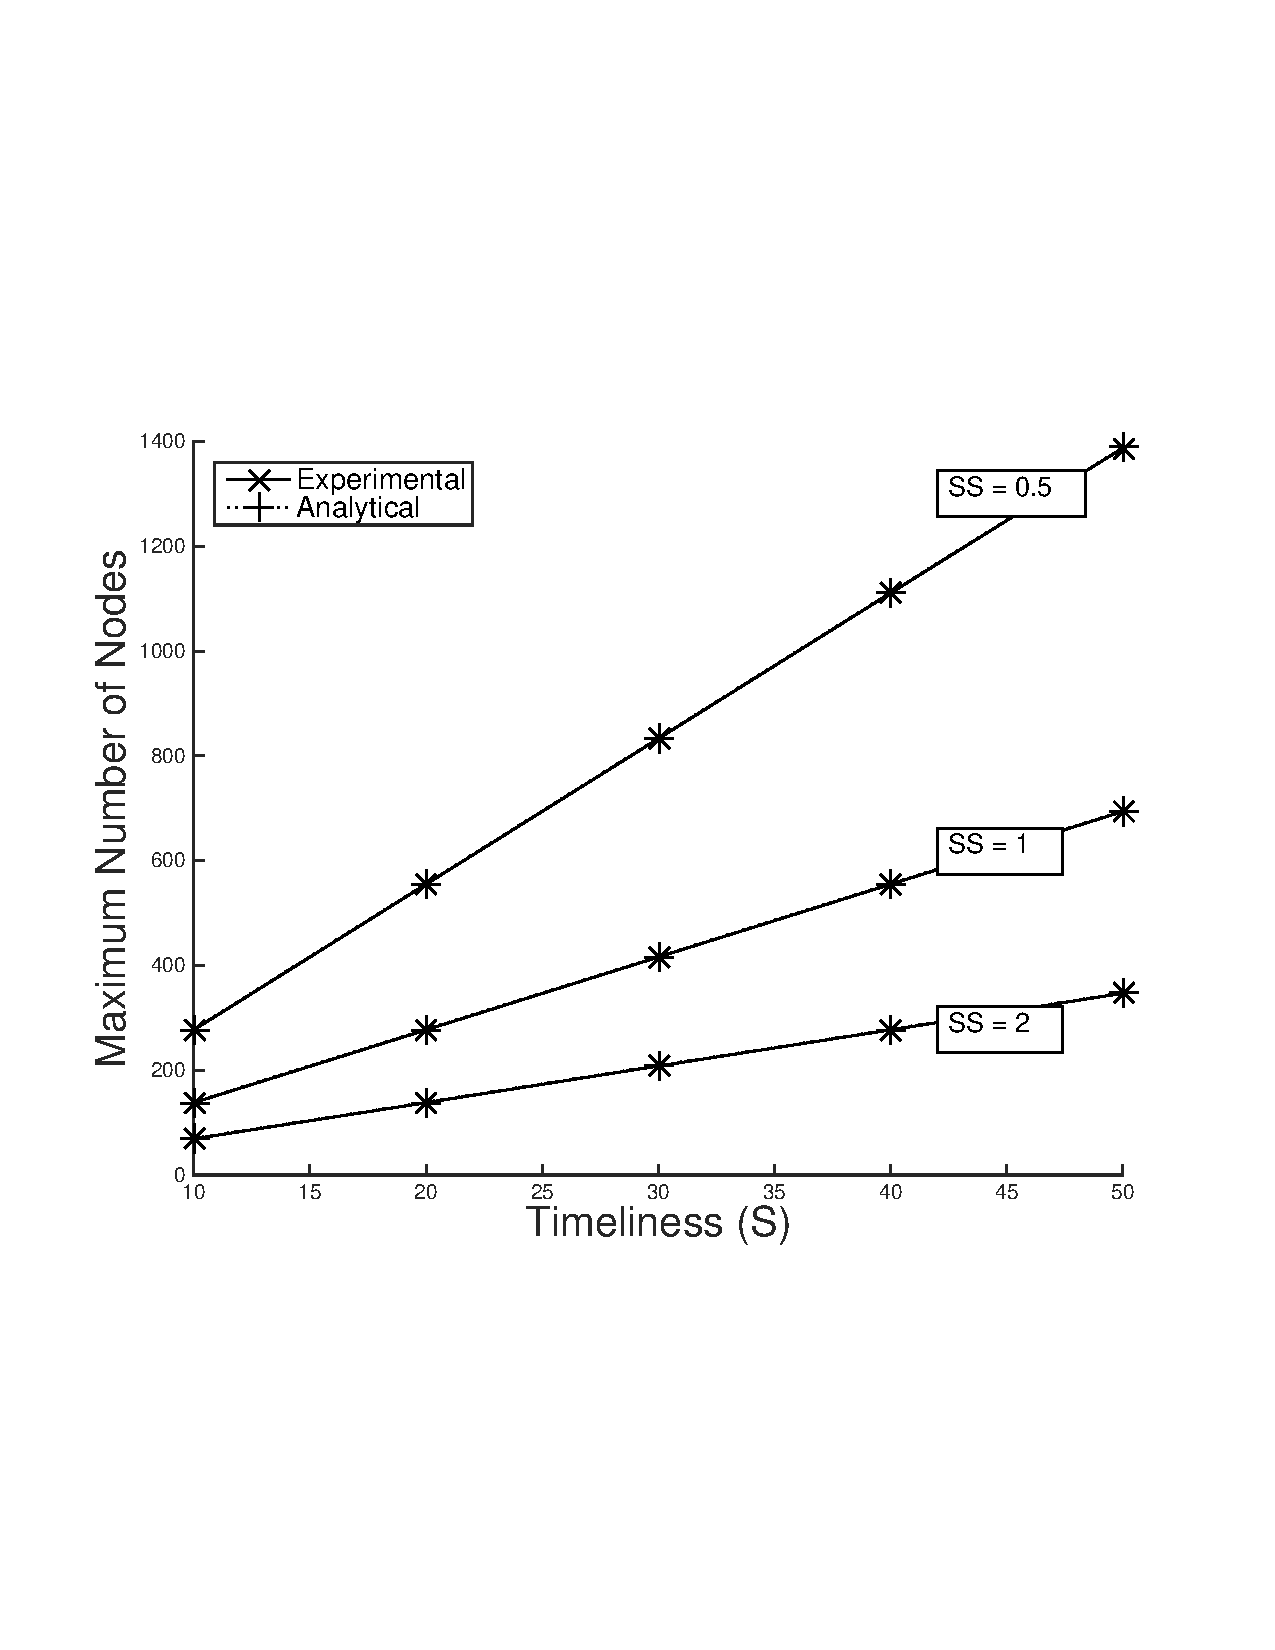
\includegraphics[scale=0.29, clip=true, trim=15mm 65mm 20mm 65mm]{clique_uni_2d.pdf}
        \label{fig:scal_vs_qoi_clique}
        }
    \subfigure[Line Network, $I_S = 12 MB$]{
        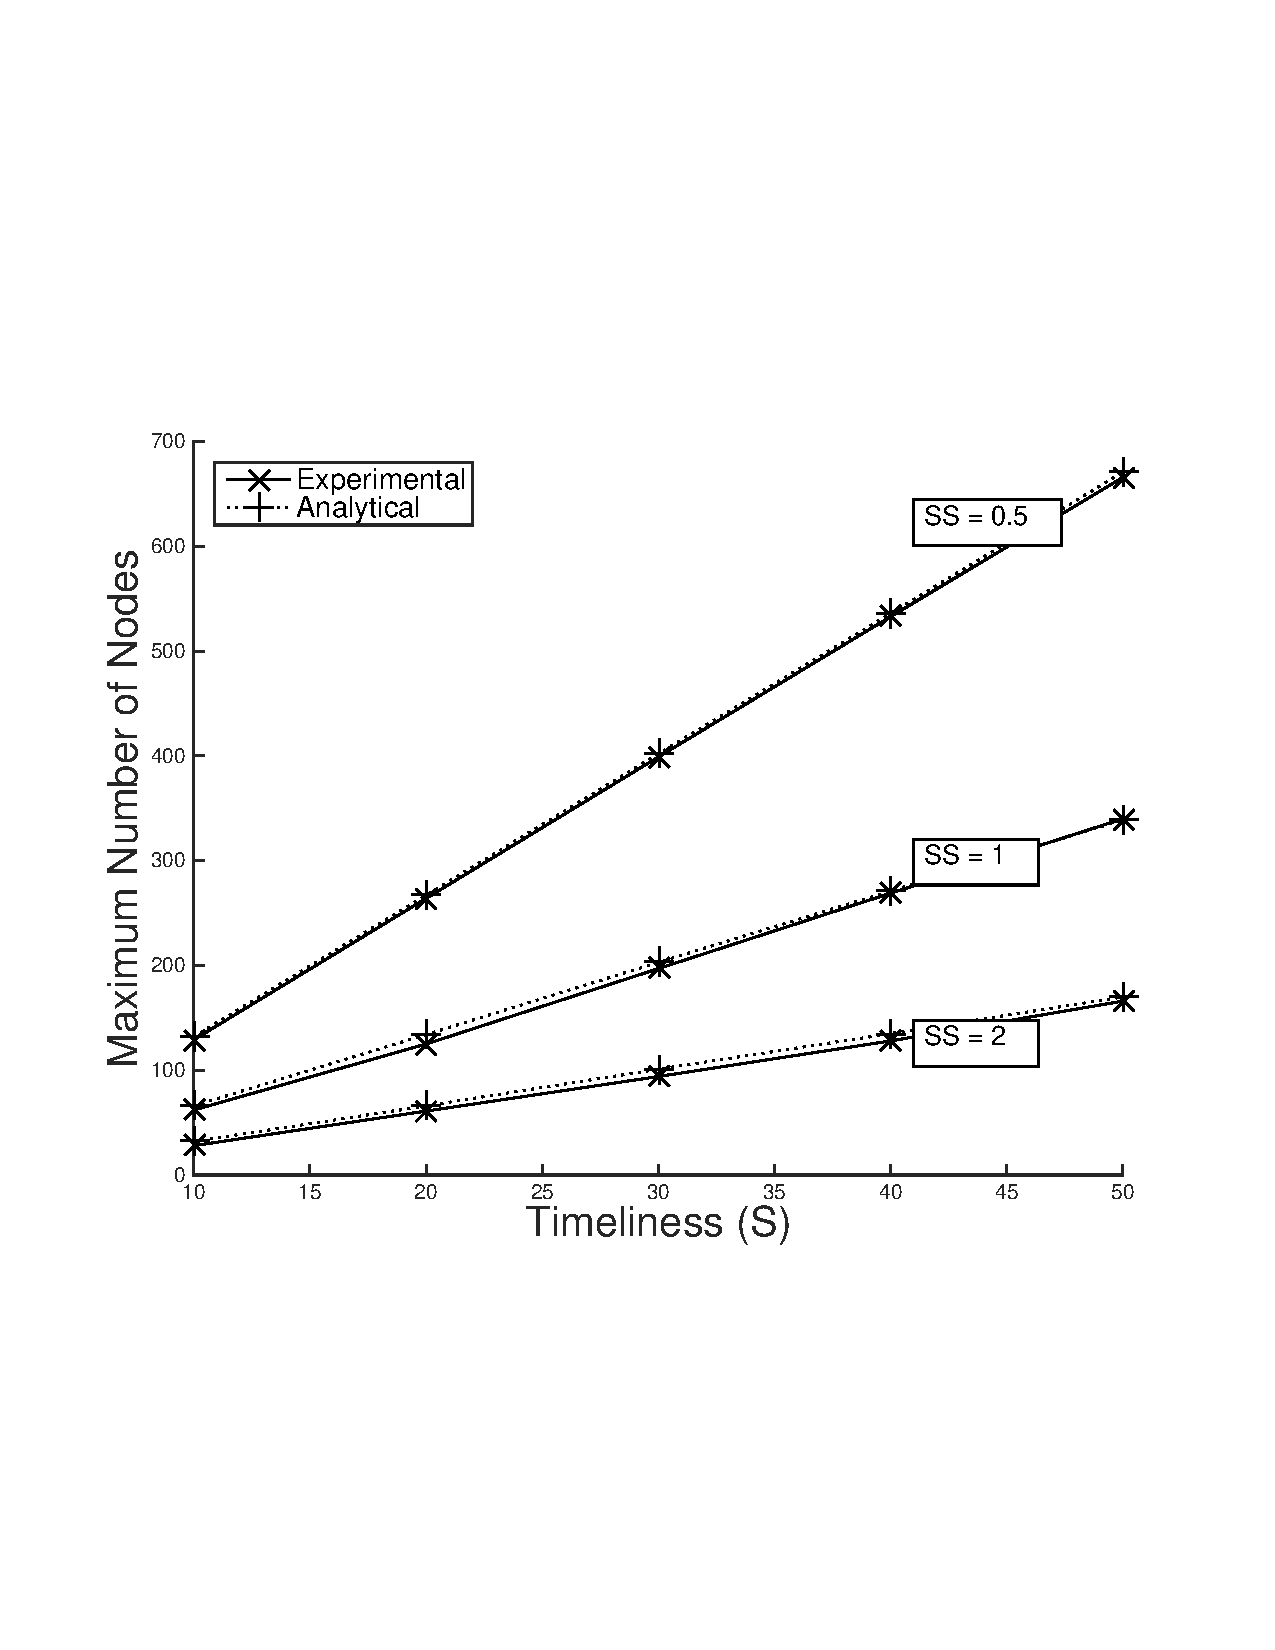
\includegraphics[scale=0.29, clip=true, trim=15mm 65mm 20mm 65mm]{line_uni_2d_mhop_2.pdf}
        \label{fig:scal_vs_qoi_line}
        }
    \subfigure[Grid Network, $I_S = 48 MB$]{
        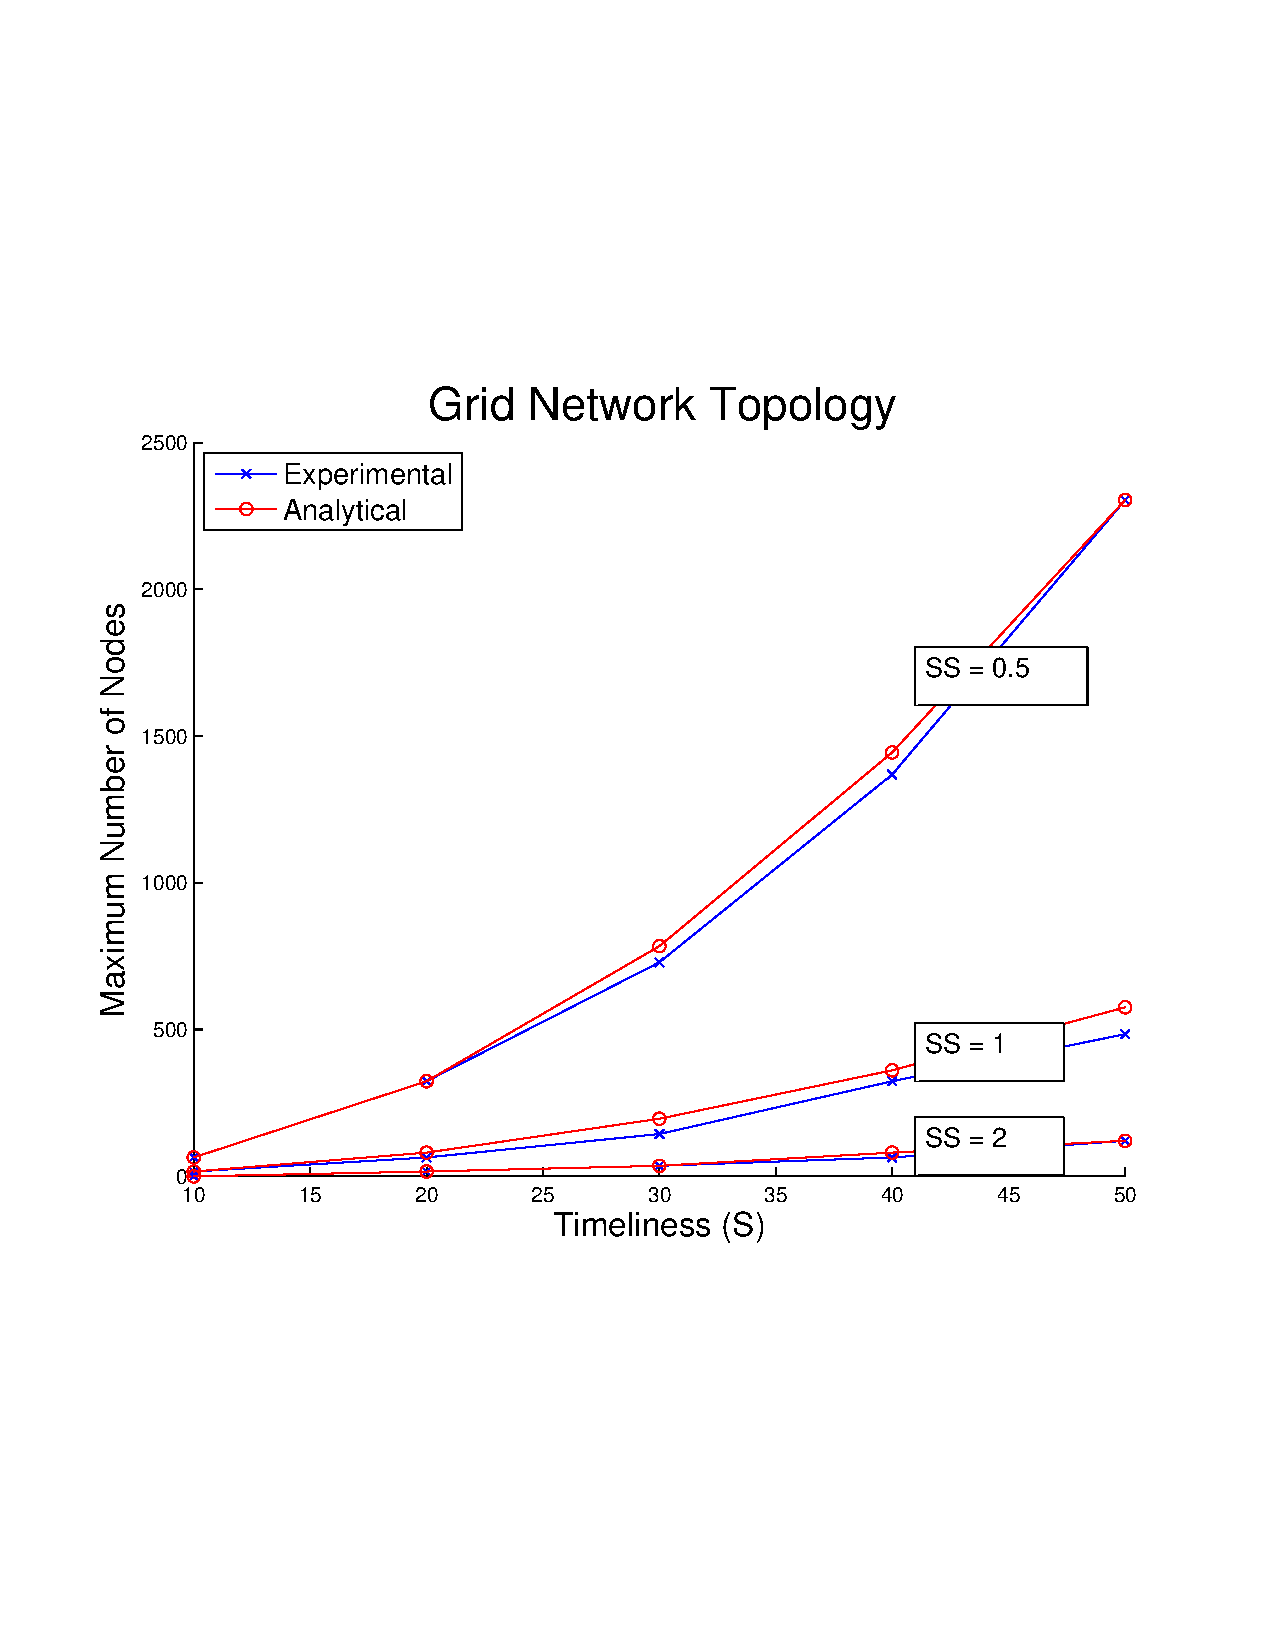
\includegraphics[scale=0.29, clip=true, trim=15mm 65mm 20mm 65mm]{grid_uni_2d_mhop_2.pdf}
        \label{fig:scal_vs_qoi_grid}
        }

   \caption{Empirical results match analytical results closely for all performed tests.  Results for each topology and a variety of sum similarity (SS) and timeliness requirements are provided.}
   \label{fig:scal_vs_qoi}

\vspace{-6mm}
\end{figure*}

\subsection{Example of Applying Framework}
\label{sec:example_apply_fw}

We illustrate the application of network signatures to the relationship in (\ref{eq:general_scal}) using an $N$-node TDMA network with three different topologies: clique, line, and grid, also known as a ``Manhattan grid.'' (Discussion of other network control protocols and topologies are addressed in Section \ref{sec:discussion}.)  We adopt a traffic model that uses Top-K queries as an example application.  We assume that all nodes have a set of collected images that are used to respond to Top-K queries.  Each node produces a query with a target image and target QoI, $\mathbf{q} = \{C, T\}$, describing the required completeness (here, we use sum similarity) and timeliness, and sends it to another node chosen at random.  The queried node will respond with the number of images, $k_{req}$, required to achieve the target sum similarity.  Values for $k_{req}$ are taken from the empirical relation in Figure \ref{fig:topkSumSim}\footnote{This application is not necessarily intended to model a known operational scenario, only a generic example to illustrate our model in a simple manner.}.  

\begin{table}[h]
\centering
\begin{tabular}{l|l|l|l|l|}
\cline{2-5}
                            					 & \textbf{CF}  					& \textbf{TF}   				& \textbf{DF}	& \textbf{PL} 			\\ \hline
\multicolumn{1}{|l|}{\textbf{Clique}} 	& N-1 							& 1                              		& 1  			& 1 					\\ \hline
\multicolumn{1}{|l|}{\textbf{Line}}   	& 3   							& $\frac{(N-1)^2}{2(N-2)}$ 	& 1.5 			& $\frac{N}{4}$			\\ \hline
\multicolumn{1}{|l|}{\textbf{Grid}}   	& 5   							& $\sqrt{N}$                       	&  2.5			& $\frac{2}{3} \sqrt{N}$   \\ \hline
\end{tabular}
\caption{CF, TF, DF, and PL values for example topologies}
\label{table:rf_ff_sf_values}
\vspace{-5mm}
\end{table}

Since our goal is to determine the point at which an average flow is no longer sustainable, we derive and use average values for $TF$, $CF$, $DF$, and $PL$ for the network.  In the case of $TF$, we use the value for the node with the largest expected $TF_i$ since flows that are routed through this node are expected to experience that largest delay and are likely to be the first that fail to meet their timeliness requirements.  Values for this example are shown in Table \ref{table:rf_ff_sf_values}, and a derivation of $TF$ for a grid network is included in Appendix \ref{sec:grid_tf_proof}.  Details about deriving the other values are explained in detail in \cite{symptotics_tech_report}.  The following equations can be used to determine QoI and network size limitations, which will be exemplified in the next two sections:

\vspace{3mm}
\noindent
Clique:
\begin{equation}
\label{eq:clique_gen}
	W \cdot T - I_S \cdot k_{req} \cdot (N-1) \geq 0
\end{equation}
Line:
\begin{equation}
\label{eq:line_gen}
	W \cdot T - 3 \cdot I_S \cdot k_{req} \cdot \frac{(N-1)^2}{N-2} - 1.5 \cdot P_S \cdot (\frac{N}{4}-1) \geq 0
\end{equation}
Grid:
\begin{equation}
\label{eq:grid_gen}
	W \cdot T - 5 \cdot I_S \cdot k_{req} \cdot \sqrt{N} - 2.5 \cdot P_S \cdot (\frac{2}{3}\sqrt{N} - 1) \geq 0
\end{equation}





\section{Results}
\label{sec:results}

In Figures \ref{fig:3dplots12} and \ref{fig:3dplots34}, we demonstrate network scalability as a function of QoI requirements for different traffic properties in a mesh setting.

\begin{figure}
\centering
    
    \subfigure[Unicast Traffic]{
        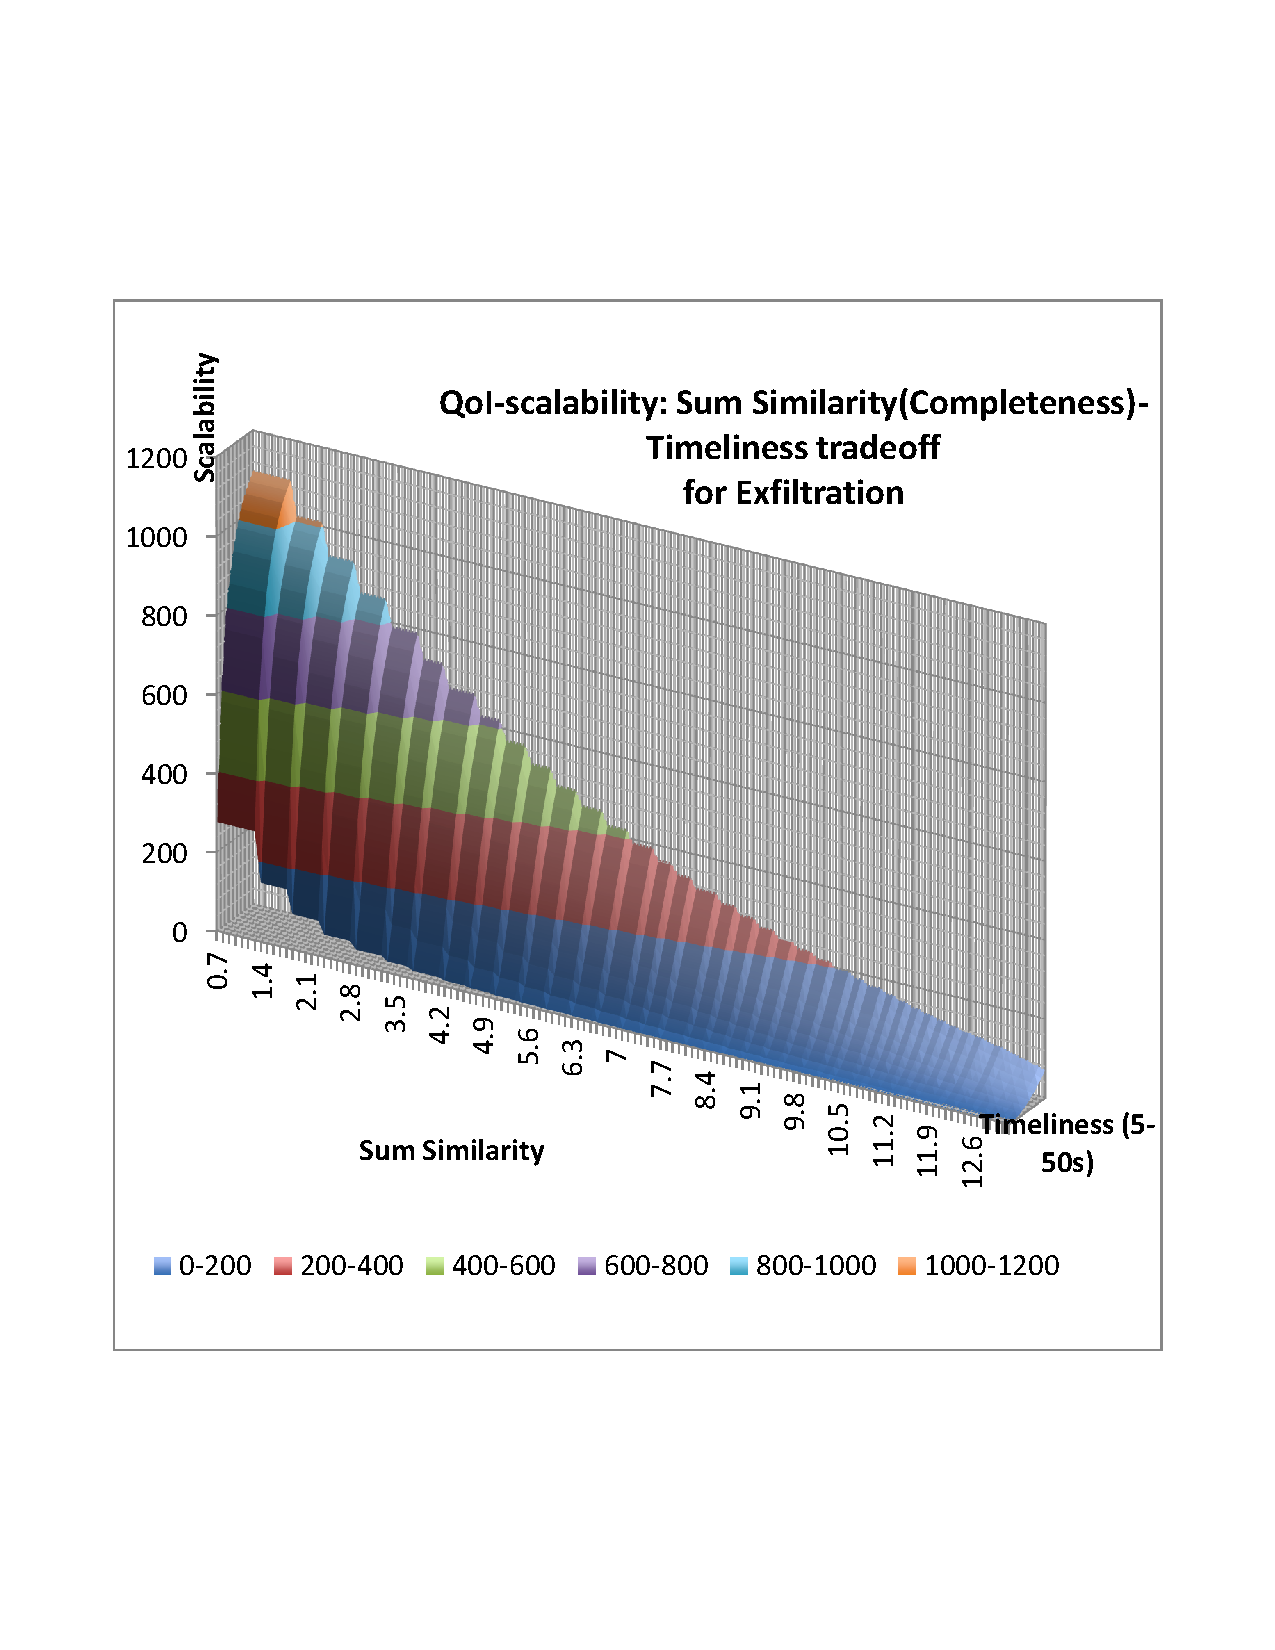
\includegraphics[scale=0.35]{figures/topk_uni.pdf}
        \label{fig:3dplot1}
        }

    \subfigure[Flooding]{
        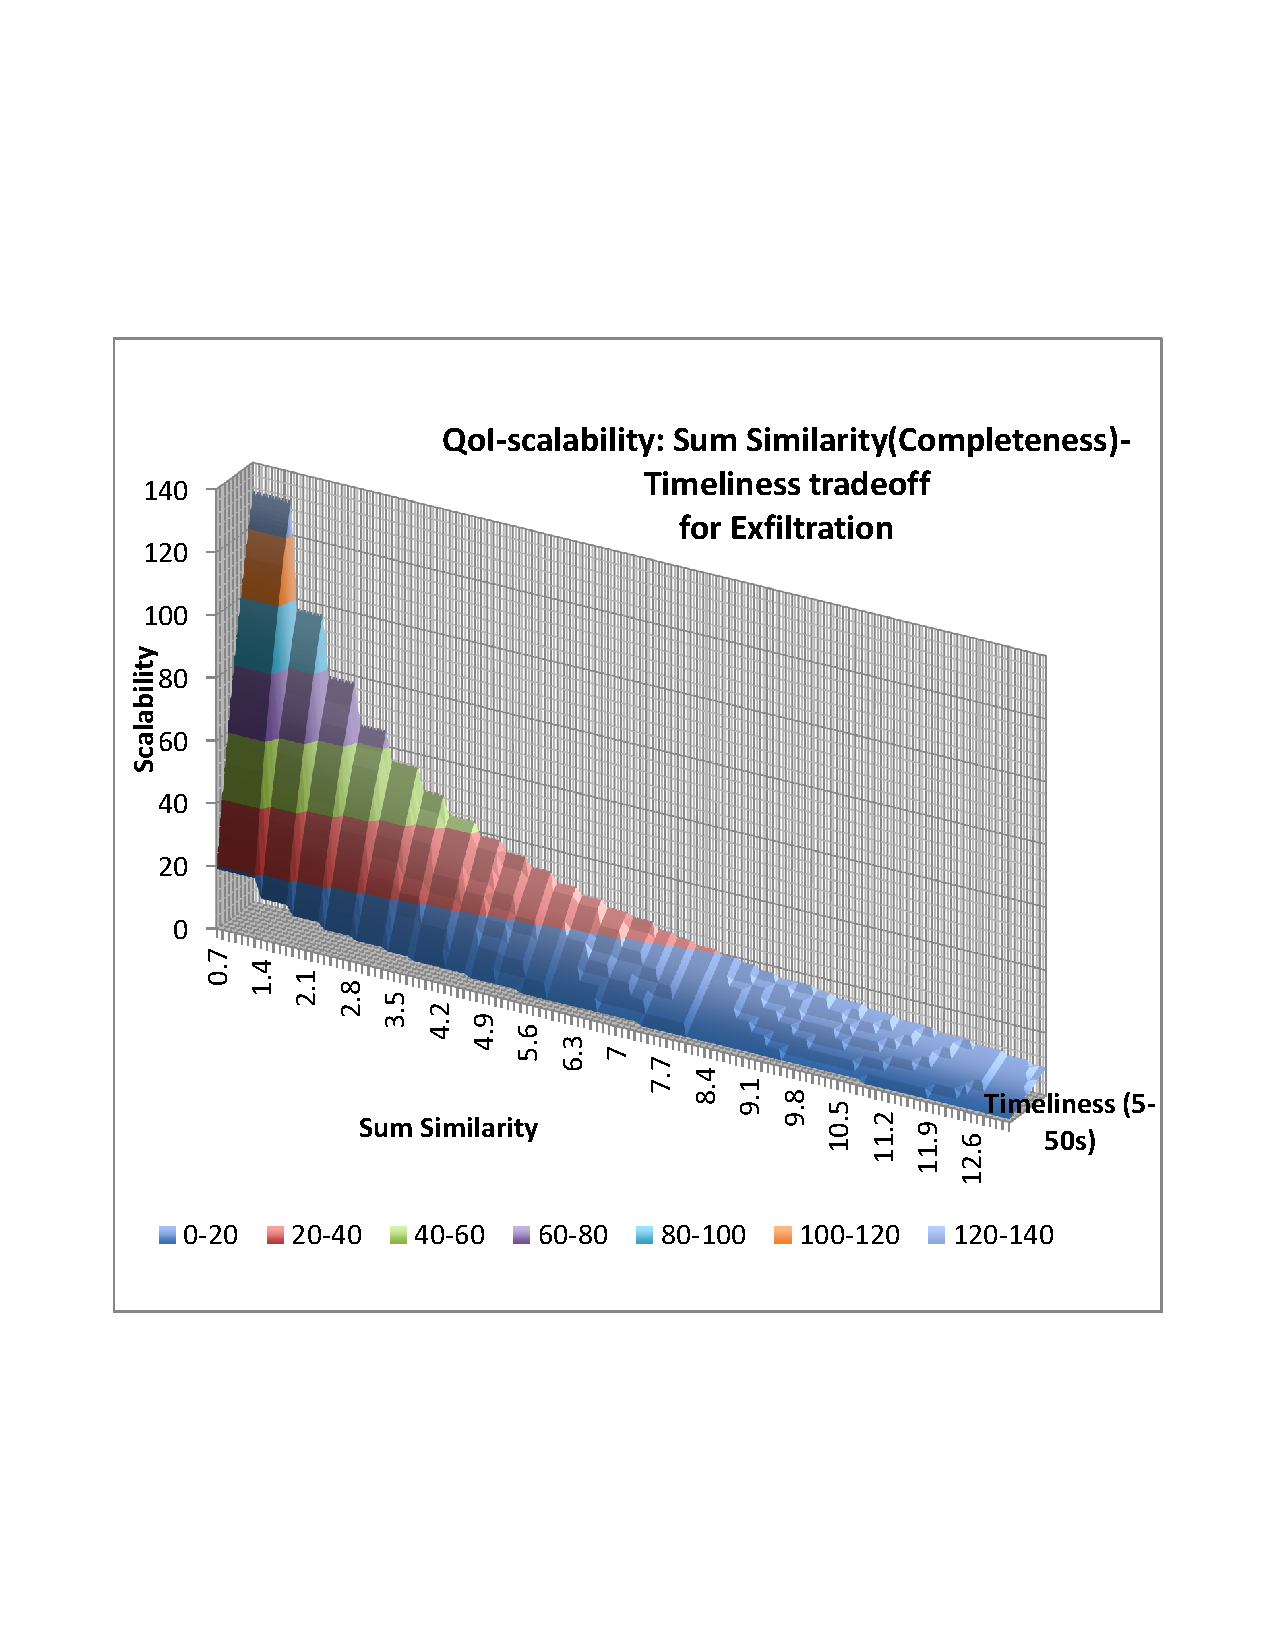
\includegraphics[scale=0.35]{figures/topk_fld.pdf}
        \label{fig:3dplot2}
        }

   \caption{Top-K:  Sum Similarity vs. Scalability vs. Timeliness}
   \label{fig:3dplots12}
\end{figure}


\begin{figure}
\centering
    \subfigure[Unicast Traffic]{
    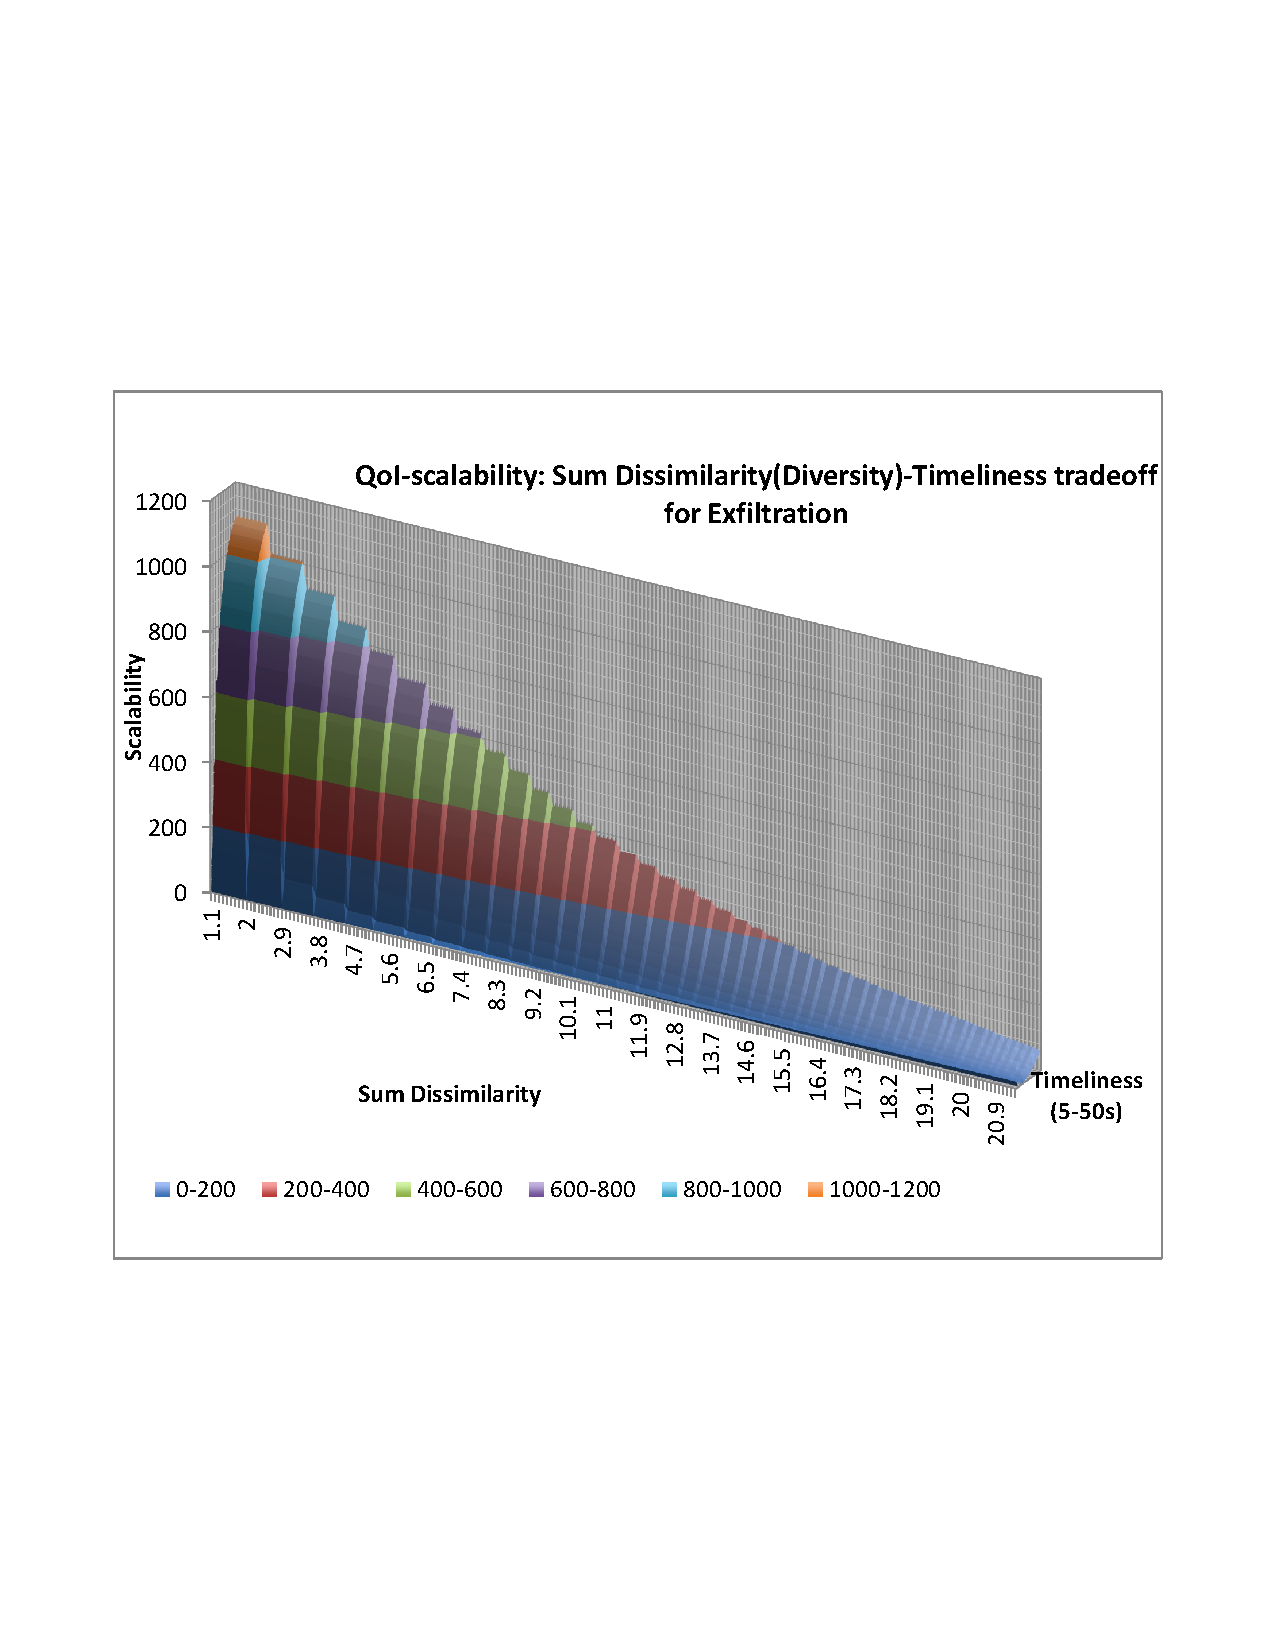
\includegraphics[scale=0.35]{figures/span_uni.pdf}
    \label{fig:3dplot3}
    }

    \subfigure[Flooding]{
    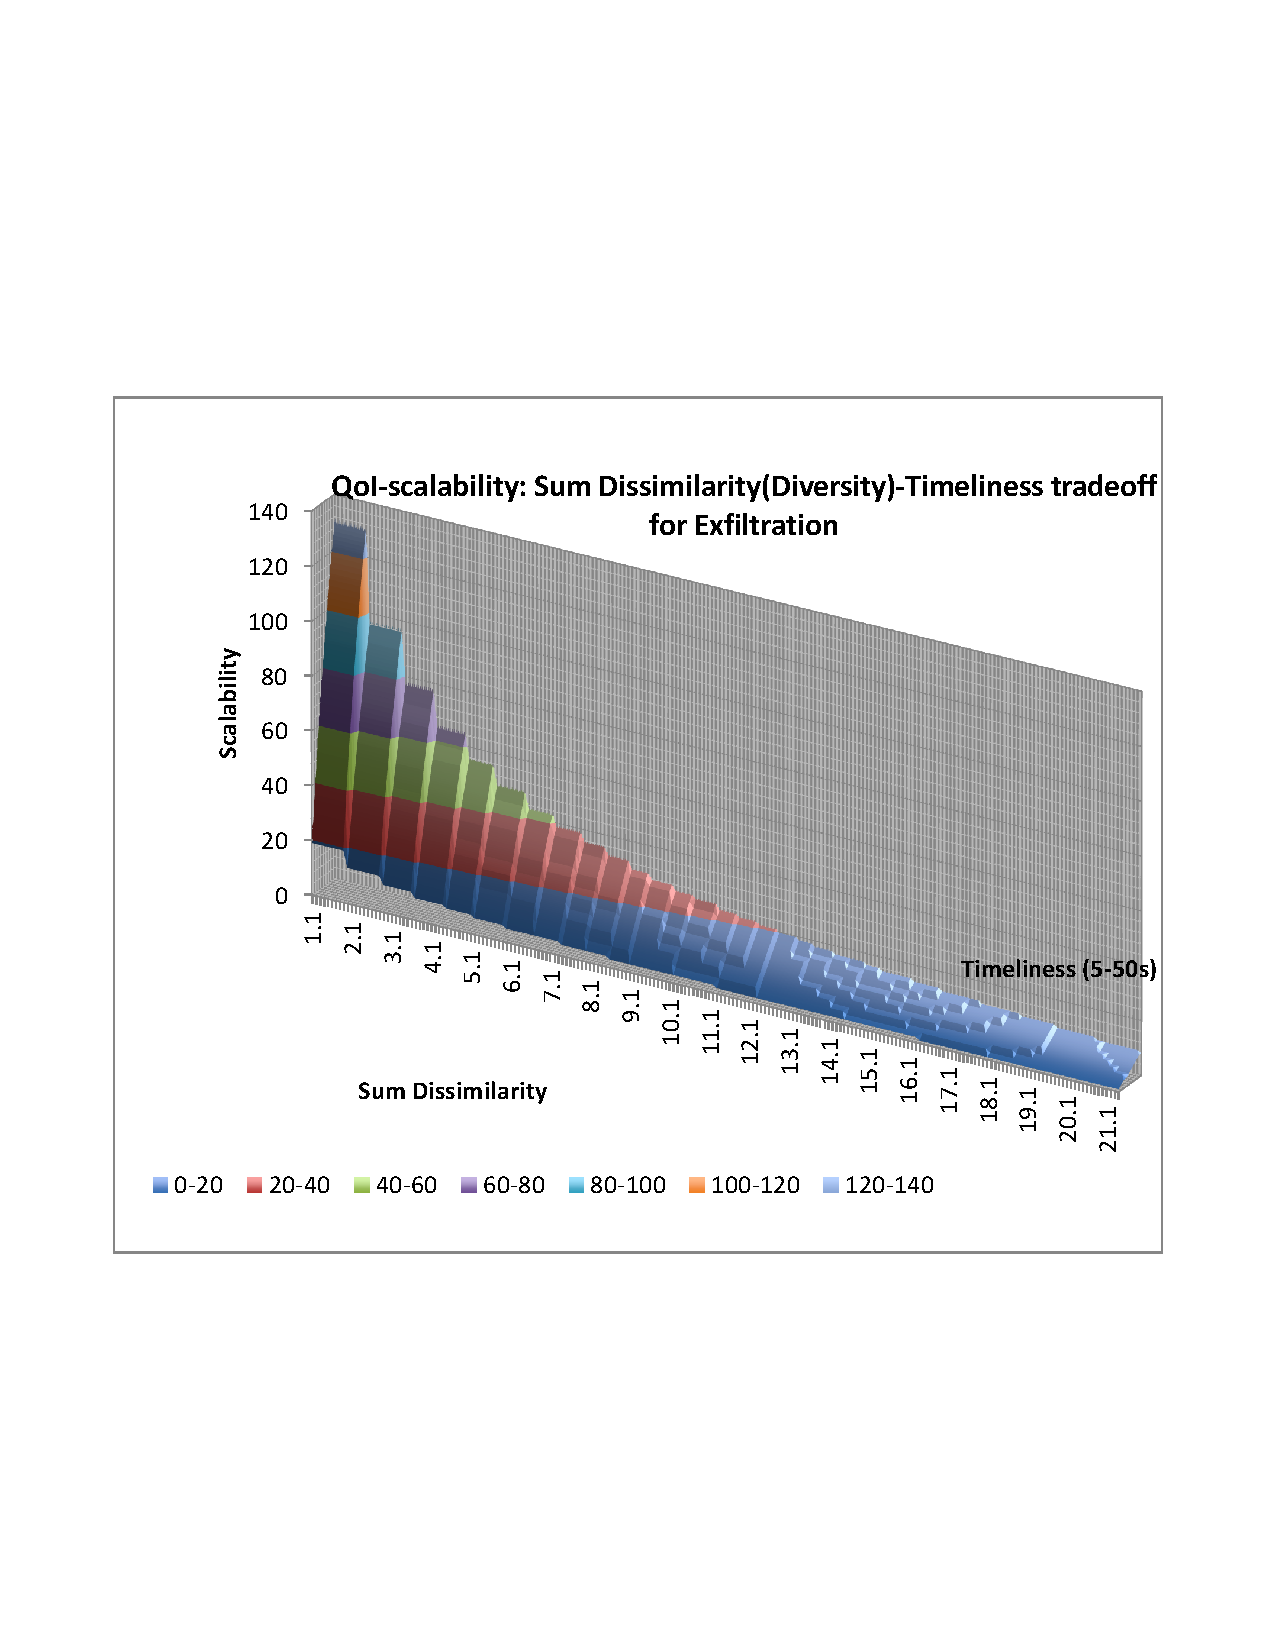
\includegraphics[scale=0.35]{figures/span_fld.pdf}
    \label{fig:3dplot4}
    }
   \caption{Spanner:  Sum Dissimilarity vs. Scalability vs. Timeliness}
      \label{fig:3dplots34}
\end{figure}

Clearly, there is a remarkable difference in the scalability depending upon
the QoI. 
The fact that QoI makes a difference is not surprising, but the {\em magnitude} of the
impact is surprising, along with the fact that there are some critical
thresholding points. Our preliminary work shows that
scalability analysis with QoI awareness has the potential to
open up new tradeoff points with
significant potential benefits in scalability. For instance, it can
potentially indicate when it makes sense to reduce QoI a bit and possibly
gain significantly in scalability (e.g. increasing timeliness constraints for small Sum Similarity/Dissimilarity values)
 %(e.g. from QoI=(10,5) to QoI=(10,10) in Figure    % These specific example points need fixed
%\ref{fig:scal-log}) 
and when such reductions will only give a marginal
increase in scalability
(e.g. increasing timeliness for high values of Sum Similarity/Dissimilarity).



\subsection{Scalably Feasible QoI Regions}
For the special case where each node possesses one image, we have observed the following dilemma. To achieve a certain level of desired QoI \text{q}, which can be defined as $(C,T)$ for Top-K queries and $(D,T)$ for spanner queries, the completeness/diversity attribute necessitates a number $K_{req}(q)$ images to be collected. When each node can contribute with at most one picture, this implies a minimum network size of $K_{req}(q)$ that is necessary for the QoI level. On the other hand, the same QoI pair also results in a maximum network size $S(q)$ from the scalability framework.
When $S(q)<K_{req}(q)$, it is not possible to provide QoI level \text{q}. Hence, we state that the QoI level \text{q} is infeasible, or \emph{scalably infeasible}.

This phenomenon defines the concept of \emph{scalably feasible QoI regions}, which define the set of QoI pairs that can be supported, given a given traffic structure. This region is given by a set of (completeness, timeliness) pairs for Top-K, and (diversity, timeliness) pairs for spanner queries. 
We demonstrate the scalably-feasible QoI regions in Figures \ref{fig:topkScalR}-\ref{fig:spanScalR}.


\begin{figure}
    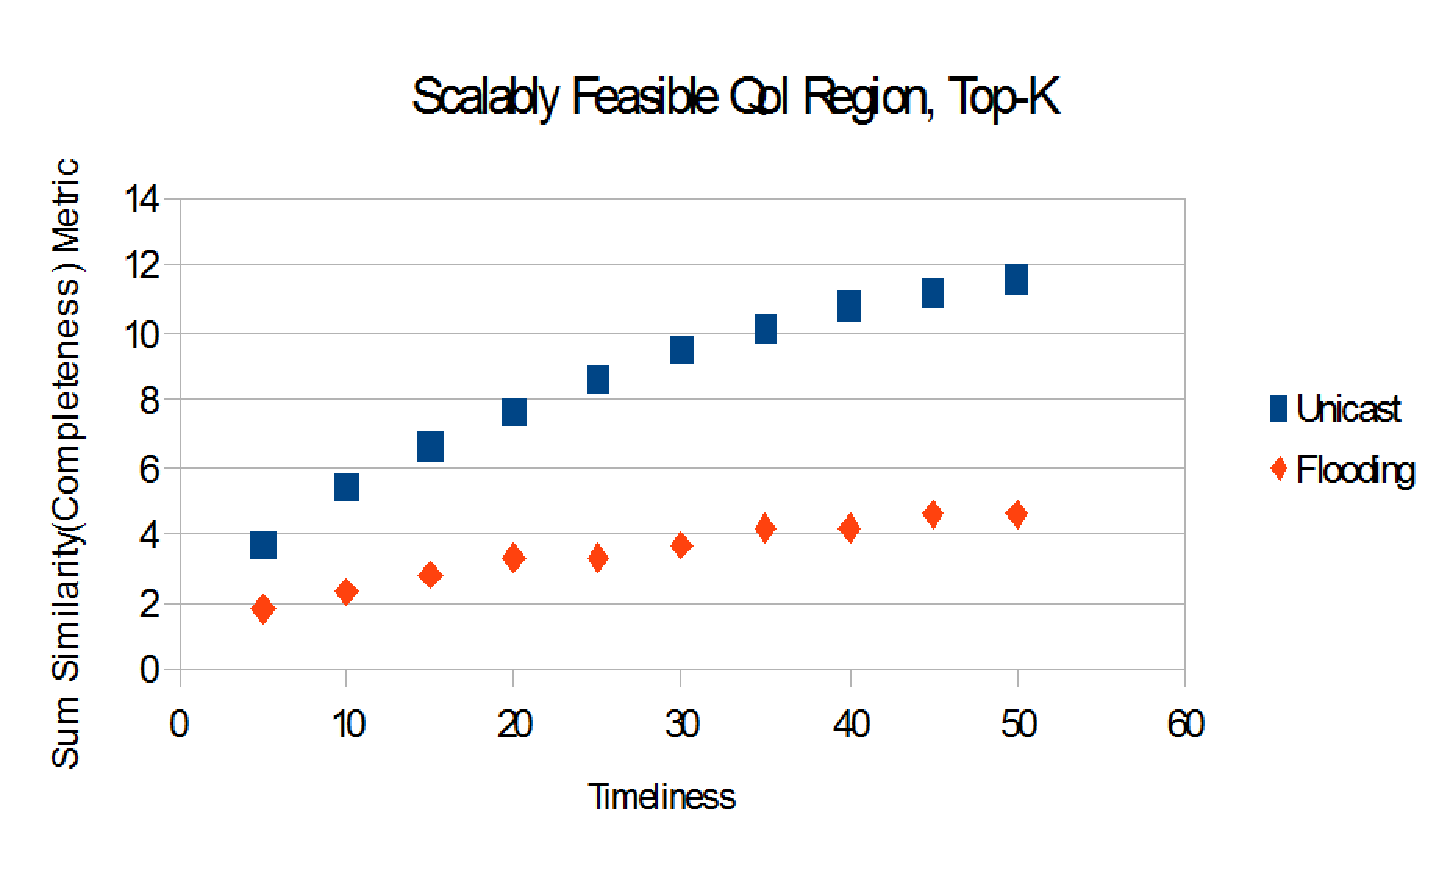
\includegraphics[scale=0.35]{figures/topkScalR.pdf}
    \caption{Feasible Scalability Region of Top-K Algorithm}
    \label{fig:topkScalR}
\end{figure}

\begin{figure}
    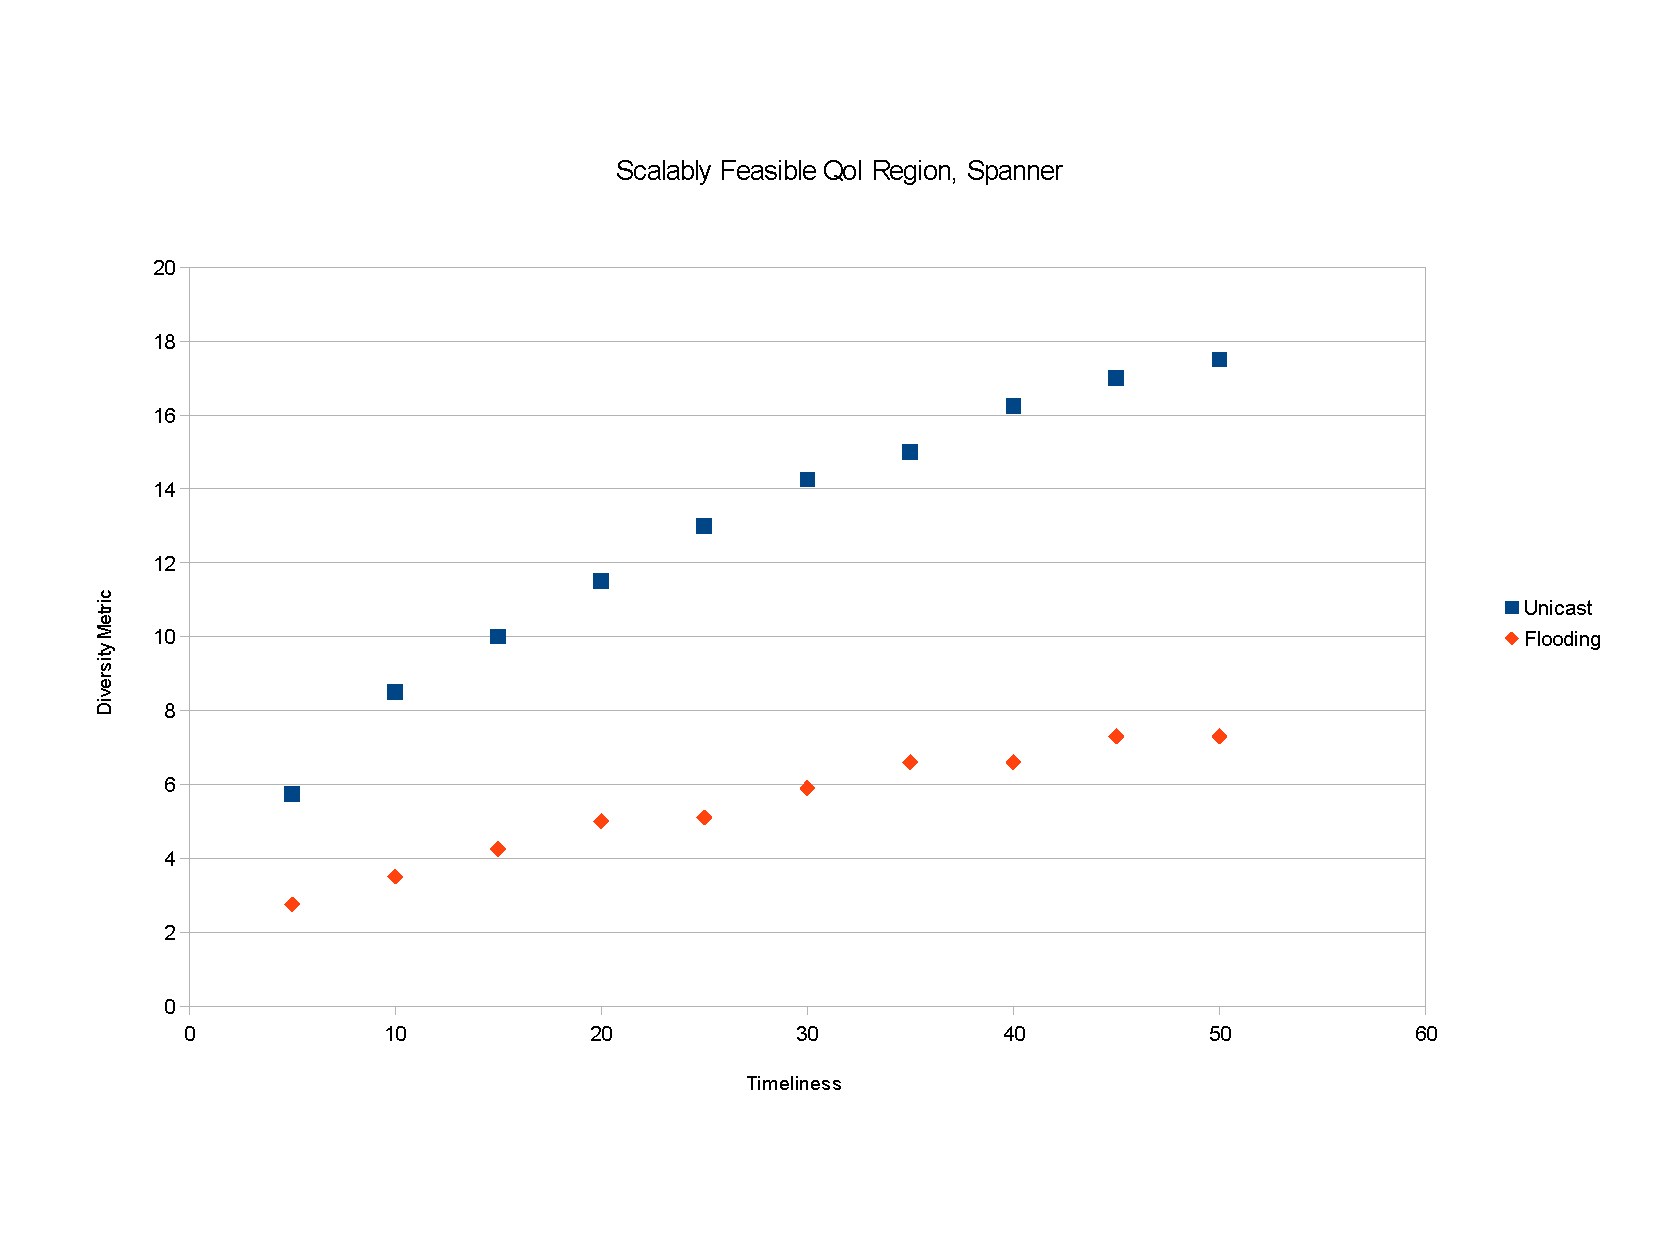
\includegraphics[scale=0.35]{figures/spanScalR.pdf}
    \caption{Feasible Scalability Region of Spanner Algorithm}
    \label{fig:spanScalR}
\end{figure}

As expected, the feasible QoI region is smaller for flooding compared with unicast. Moreover, these regions clearly demonstrate the tradeoff between the completeness/diversity that can be obtained and the timeliness that can be tolerated. 



\section{Conclusion}
\label{sec:conclusion}

Wrap it up with the highlights/takeaways.  Maybe also include future work.


% conference papers do not normally have an appendix


% use section* for acknowledgement
%\section*{Acknowledgment}


%The authors would like to thank...


% trigger a \newpage just before the given reference
% number - used to balance the columns on the last page
% adjust value as needed - may need to be readjusted if
% the document is modified later
%\IEEEtriggeratref{8}
% The "triggered" command can be changed if desired:
%\IEEEtriggercmd{\enlargethispage{-5in}}

% references section

% can use a bibliography generated by BibTeX as a .bbl file
% BibTeX documentation can be easily obtained at:
% http://www.ctan.org/tex-archive/biblio/bibtex/contrib/doc/
% The IEEEtran BibTeX style support page is at:
% http://www.michaelshell.org/tex/ieeetran/bibtex/
%\bibliographystyle{IEEEtran}
% argument is your BibTeX string definitions and bibliography database(s)
%\bibliography{IEEEabrv,../bib/paper}
%
% <OR> manually copy in the resultant .bbl file
% set second argument of \begin to the number of references
% (used to reserve space for the reference number labels box)
%\begin{thebibliography}{1}


\bibliographystyle{unsrt}

\bibliography{references}

%\bibitem{IEEEhowto:kopka}
%H.~Kopka and P.~W. Daly, \emph{A Guide to \LaTeX}, 3rd~ed.\hskip 1em plus
%  0.5em minus 0.4em\relax Harlow, England: Addison-Wesley, 1999.

%\end{thebibliography}




% that's all folks
\end{document}


